\documentclass[a4paper,10pt]{article}

\usepackage[backend=biber]{biblatex}
\bibliography{solutions_bibliography}

\usepackage[dvipsnames,table]{xcolor}
\usepackage{amsmath}
\usepackage{amssymb}
\usepackage{gensymb}
\usepackage{amsthm}
\usepackage{microtype}
\usepackage{adjustbox}
\usepackage[hidelinks]{hyperref}
\usepackage[parfill]{parskip}
\usepackage{exercises}
\usepackage{pgfplots}
\usepgfplotslibrary{polar}
\usepackage{graphicx}
\usepackage{sidecap}
\sidecaptionvpos{figure}{c}
\usepackage{float}
\usepackage{eufrak}
\usepackage{polynom}
\usepackage{mdframed}
\usepackage{mathtools}
\usepackage{commath}

\newtheorem*{thm}{Theorem}
\newtheorem*{iden}{Identity}
\newtheorem*{lemma}{Lemma}
\newtheorem*{axiom}{Axiom}
\newtheorem*{defn}{Definition}
\DeclareMathOperator{\cis}{cis}
\DeclareMathOperator{\carg}{arg}
\newcommand*\realp[1]{ \mathfrak{Re} \left ( {#1} \right )  }
\newcommand*\imagp[1]{ \mathfrak{Im} \left ( {#1} \right )  }

\begingroup
    \makeatletter
    \@for\theoremstyle:=definition,remark,plain\do{%
        \expandafter\g@addto@macro\csname th@\theoremstyle\endcsname{%
            \addtolength\thm@preskip\parskip
            }%
        }
\endgroup

\usepackage[inline]{enumitem}

\def\signed #1{{\leavevmode\unskip\nobreak\hfil\penalty50\hskip2em
  \hbox{}\nobreak\hfil(#1)%
  \parfillskip=0pt \finalhyphendemerits=0 \endgraf}}

\pgfplotsset{
  /pgfplots/xlabel near ticks/.style={
     /pgfplots/every axis x label/.style={
        at={(ticklabel cs:0.5)},anchor=near ticklabel
     }
  },
  /pgfplots/ylabel near ticks/.style={
     /pgfplots/every axis y label/.style={
        at={(ticklabel cs:0.5)},rotate=90,anchor=near ticklabel}
     }
  }

\newsavebox\mybox
\newenvironment{aquote}[1]
  {\savebox\mybox{#1}\begin{quote}}
  {\signed{\usebox\mybox}\end{quote}}
\newcommand{\hard}{\refstepcounter{enumi}\item[$^\star$\theenumi.]}
\newcommand{\answer}{\bfseries\color{Emerald}\refstepcounter{enumi}\item[\theenumi.]}
\newcommand{\answerb}{\bfseries\color{Emerald}\refstepcounter{enumii}\item[\theenumii.]}

\title{\color{Emerald}Solutions to Solutions\\\small{Sample Answers to the Exercises}}
\author{Alex Elzenaar}%\\Upper Hutt College}
\date{\today}

\begin{document}

\maketitle
\tableofcontents

\clearpage
\section{Introduction}
This booklet consists of worked solutions to all exercises in \textit{Solutions}. Please
check the date on the cover of both texts and ensure it matches. They are designed to be
read in conjunction with the main text.

Note that these solutions are most definitely not the only possible solutions! They are only
indicative of what a solution to the problem could look like.

\subsection*{Notation}
We use standard set notation: $ \mathbb{N} $ stands for the natural numbers (excluding zero), $ \mathbb{Z} $ for
the integers, $ \mathbb{Q} $ for the rationals, $ \mathbb{R} $ for the reals, and $ \mathbb{C} $ for the complex
numbers. The symbol $ \in $ is the set inclusion symbol, and $ \subseteq $ is the subset symbol.

Sigma notation is also occasionally used: the notation
\begin{displaymath}
  \sum^{N}_{n = 0} f(n)
\end{displaymath}
means the sum $ f(0) + f(1) + \cdots + f(N) $. If $ \sum $ is replaced by $ \prod $, the intended meaning is $ f(0) f(1) \cdots f(N) $.

\subsection*{Definitions}
I apologise for using the following definitions occasionally without explanation:
\begin{itemize}
  \item \textbf{Group:} A number system with one operation that is invertible, such that there is an identity. Example: the integers
                        together with addition (the identity being the number 1).
  \item \textbf{Ring:}  A number system in which we can carry out the operations of addition, subtraction, and multiplication. Example: the integers.
  \item \textbf{Field:} A number system in which we can carry out the operations of addition, subtraction, multiplication, and division. Example: the real
                        numbers.
\end{itemize}

\subsection*{Induction}
\begin{axiom}[The Axiom of Induction]
  Let $ S $ be a set. Then if $ 1 \in S $, and if $ n \in S $ then $ n + 1 \in S $, we must have $ \mathbb{N} \subseteq S $.
\end{axiom}
In other words, if a set contains 1, and it contains $ n + 1 $ whenever it contains $ n $, then it contains all natural numbers.
This is often an easy way to prove that a statement holds for all natural numbers (and, in fact, integers). We occasionally make
use of it here,\footnote{~Like real adults, we often leave the actual induction proof to the reader (in general it is obvious
what the base and inductive steps look like.)} although we usually give an alternative proof without using induction. If one is
interested, this is a standard proof technique and is thus easily Googleable.

I give the following standard example of induction:
\begin{thm}
  The sum of the first $ n $ natural numbers is $ \frac{n(n+1)}{2} $.
\end{thm}
\begin{proof}
  Consider the case $ n = 1 $. Then the formula gives us $ \frac{1(1 + 1)}{2} = 1 $, which is correct.

  Now, suppose the formula gives us the correct result for $ n $. Then:
  \begin{displaymath}
    \frac{(n+1)(n+2)}{2} = \frac{n(n+1) +2(n + 1)}{2} = \frac{n(n+1)}{2} + (n + 1)
  \end{displaymath}
  so the formula gives us the correct result for $ n + 1 $.

  Hence, by the principle of induction, the set of all natural numbers is a subset of the set of all $ n $ for
  which the formula holds true; so the formula works for all $ n \in \mathbb{N} $.
\end{proof}

\subsection*{Recommended Further Reading}
On algebra, I would recommend Charles C. Pinter's \textit{A Book of Abstract Algebra} for the beginner (although I much
prefer Michael Artin's \textit{Algebra}, it is not as accessible for a high-school audience). On proof techniques and
basic concepts of set theory and number theory, I recommend Kevin Houston's \textit{How to Think Like a Mathematician}.

Of course, the books in the bibliography are recommended as well --- but most of them require more sophisticated mathematical
knowledge to be accessible and so the reader is kindly advised not to touch (for example) the textbooks on Galois Theory without
consulting a professional! Ian Stewart's \textit{Taming the Infinite} is recommended for the casual audience.

\let\oldsection\section
\renewcommand\section{\clearpage\oldsection}

\section{Quadratic Equations}
\begin{enumerate}
  \answer Find an example of a \textbf{quadratic equation} with the solutions:
        \begin{enumerate}
          \answerb $ x = 7 $ and $ x = 4 $
          \answerb $ x = 7 $ and $ x = -4 $
          \answerb $ x = -7 $ and $ x = -4 $
          \answerb Only $ x = 3 $
        \end{enumerate}
\end{enumerate}

\begin{gather*}
  0 = (x-7)(x-4) = x^2 - 11x + 28,\\
  0 = (x-7)(x+4) = x^2 -3x - 28,\\
  0 = (x+7)(x+4) = x^2 + 11x + 28, \text{ and}\\
  0 = (x-3)^2 = x^2 - 6x + 9.
\end{gather*}

All constant multiples of these will also have the same roots.

\filbreak\begin{enumerate}[resume]
  \answer Use the discriminant $ \Delta_2 $ of the following quadratics to find the
        number of distinct real roots each one has, without explicitly calulating
        those roots.
        \begin{enumerate}
          \answerb $ 3x^2 + 6x + 3 = 0 $
          \answerb $ x^2 + 10x + 1 = 0 $
          \answerb $ x^2 + 5x + 9 = 0 $
          \answerb $ x^2 - \frac{14x}{3} + \frac{49}{9} = 0 $
        \end{enumerate}
\end{enumerate}

Recall that the quadratic discriminant $ \Delta_2 = b^2 - 4ac $ will "discriminate"
between the three possibilities (two real roots, one repeated real root, or no real
root).

For (a), $ \Delta_2 =  6^2 - 4\cdot4\cdot9 = 0 $, so the first equation has one repeated real root.
For (b), $ \Delta_2 =  10^2 - 4 > 0 $, so the second equation has two distinct real roots.
For (c), $ \Delta_2 = 5^2 - 4\cdot9 < 0 $, so the third equation has no real roots.

We multiply the fourth equation in (d) by 9 to clear the fractions and simplify our calculations.
We then have $ \Delta_2 = (-42)^2 - 4\cdot9\cdot49 = 0 $, so it has one repeated real root.

\filbreak\begin{enumerate}[resume]
  \answer Use the \emph{difference of two squares} identity $ x^2 - b^2 = (x-b)(x+b) $ to factorise and hence
        solve the following equations for $ x $:
        \begin{enumerate}
          \answerb $ x^2 - 9 = 0 $
          \answerb $ x^2 - 7 = 0 $
          \answerb $ x^2 - 15 = 1 $
          \answerb $ x^2 - 2ab = a^2 + b^2 $
        \end{enumerate}
\end{enumerate}

$ x^2 - 9 = (x+3)(x-3) $, so $ x = \pm 3 $;\\
$ x^2 - 7 = (x+\sqrt{7}){x-\sqrt{7}} $, so $ x = \pm \sqrt{7} $;\\
$ x^2 - 16 = (x + 4)(x-4) $, so $ x = \pm 4 $; and\\
$ x^2 - a^2 - 2ab - b^2 = x^2 - (a+b)^2 = (x + a + b)(x - a - b) $, so $ x = \pm (a+b) $.


\filbreak\begin{enumerate}[resume]
  \answer Prove that $ ax^2 + bx + c = Ax^2 + Bx + C $ implies that $ a = A $, $ b = B $, and $ c = C $.
        This result allows us to \textit{match coefficients}, an important tool which we can use to
        reason about the symmetries of polynomials.
\end{enumerate}
Both polynomials agree everywhere, so in particular they agree at $ x = 0 $. By direct
substitution, we have therefore got that $ c = C $. Hence $ ax^2 + bx = Ax^2 + Bx $.
These polynomials agree at $ x = 1 $, so $ a + b = A + B $; similarly, these polynomials
agree at $ x = -1 $ and so $ a - b = A - B $. Adding, $ 2a = 2A \implies a = A $;
by subtraction, $ 2b = 2B \implies b = B $.

\filbreak\begin{enumerate}[resume]
  \answer Show that if $ \alpha $ and $ \beta $ are the two solutions of $ x^2 + bx + c = 0 $, then
        we have $ -b = \alpha + \beta $ and $ c = \alpha\beta $.
\end{enumerate}
We simply match coefficients: $ x^2 + bx + c = (x - \alpha)(x - \beta) = x^2 - (\alpha + \beta)x + \alpha\beta $.

\filbreak\begin{enumerate}[resume]
  \answer Factorise $ x^2 - 3x - 40 $ by inspecting the coefficients and using the
        identity that a quadratic with the two solutions $ a $ and $ b $ is given
        by $ (x-a)(x-b) = x^2 -(a+b)x + ab $ (note the change of sign in the factors).
\end{enumerate}

We have that $ ab = -40 $ and $ a + b = 3 $. We know that $ 5 \times 8 = 40 $ - and
$ 5 - 8 = -3 $. Hence $ b = 8 $ and $ a = -5 $.

\filbreak\begin{enumerate}[resume]
  \answer For which values of $ k $ does the graph of the quadratic function
        $ y = x^2 +(3k-1)x + (2k+10) $ not touch the $ x$-axis?
\end{enumerate}

We need $ \Delta_2 < 0 $. $ \Delta_2 = (3k - 1)^2 - 4(2k+10) = 9k^2 - 14k - 39 $,
and using the quadratic formula we have the two solutions for this as $ k = 3 $
and $ k = -\frac{13}{9} $. Since our polynomial for $ \Delta_2 $ is concave up (positive
coefficent on the $ x^2 $ term), $ \Delta_2 < 0 $ for $ -\frac{19}{3} < k < 3 $.

\filbreak\begin{enumerate}[resume]
  \answer Do the zeroes of a function uniquely identify that function? Why/why not?
\end{enumerate}

It is easily seen that given $ n $ roots $ x_0,x_1,...,x_n $, one polynomial with those
roots will be $ y = (x - x_0)(x - x_1)...(x - x_n) $. However, we also see that
$ y = K(x - x_0)(x - x_1)...(x - x_n) $ (where $ K \neq 0 $ is an arbitrary constant) has
exactly those roots as well (when $ y = 0 $, $ K $ can be divided out). So the
zeroes of a function do not uniquely identify the function.

\filbreak\begin{enumerate}[resume]
  \answer Solve the following equations in the real numbers:
        \begin{enumerate*}
          \answerb $ w^4 + 30w^2 + 29 = 0 $, and
          \answerb $ 3 e^{2x} - 24 e^x - 8 = 0 $.
        \end{enumerate*}
\end{enumerate}

The first equation is a quadratic in $ w^2 $, so $ w^2 = -1 $ and $ w^2 = -29 $
(by inspection or by the quadratic formula); hence this equation has no solutions
in the real numbers.

$ e^{2x} = \left(e^x\right)^2 $ so the second formula is a quadratic in $ e^x $.
Solving this with the quadratic formula, we obtain $ e^x = \frac{12 \pm 2\sqrt{42}}{3} $.
Since we cannot yet take the logarithm of a negative number, the only solution is
$ x = \ln{\frac{12 +m 2\sqrt{42}}{3}} $.

\filbreak\begin{enumerate}[resume]
  \answer Write each of the following in the form $ (x + p)^2 = q $ for some $ p $ and $ q $, and hence find their
        solutions by completing the square.
        \begin{enumerate}
          \answerb $ x^2 - 3x + 4 = 0 $
          \answerb $ x^2 - 6x - 10 = 0 $
          \answerb $ x^2 - 26x + 47 = 0 $
          \answerb $ 6x^2 - 12x + 13 = 0 $
          \answerb $ -2x^2 + 3x + 5 = 0 $
        \end{enumerate}
\end{enumerate}
\begin{align*}
  x^2 - 3x + 4 = 0 \implies (x - \tfrac{3}{2})^2 - \tfrac{7}{4} &\implies x = \pm\sqrt{\tfrac{7}{4}} + \tfrac{3}{2}\\
  x^2 - 6x - 10 = 0 \implies (x - 3)^2 = 19 &\implies x = \pm\sqrt{19} + 3\\
  x^2 - 26x + 47 = 0 \implies (x - 13)^2 = 122 &\implies x = \pm\sqrt{122} + 13\\
  6x^2 - 12x + 13 = 0 \implies x^2 - 3x + \frac{13}{6} = 0 \implies (x - \tfrac{3}{2})^2 = \tfrac{1}{12} &\implies x = \pm\sqrt{\tfrac{1}{12}} + \tfrac{3}{2}\\
  -2x^2 + 3x + 5 = 0 \implies x^2 - \tfrac{3}{2} x - \tfrac{5}{2} = 0 \implies (x - \tfrac{3}{4})^2 = \tfrac{49}{16} &\implies x = \tfrac{3}{4}\pm\tfrac{7}{4}
\end{align*}

\filbreak\begin{enumerate}[resume]
  \answer Suppose that $ x^2 + bx + c = 0 $ has two roots, $ \alpha $ and $ \beta $.
        \begin{enumerate}
          \answerb Show that $ \alpha^2 + \beta^2 = b^2 - 2c $.
          \answerb Show that $ \Delta_2 \left[x^2 + bx + c\right] = (\alpha - \beta)^2 $.
        \end{enumerate}
\end{enumerate}
\paragraph{(a)}
We have that $ x^2 + bx + c = (x - \alpha)(x - \beta) = x^2 - (\alpha + \beta)x + \alpha\beta $,
so $ \alpha + \beta = -b $. Hence $ b^2 = (\alpha + \beta)^2 = \alpha^2 + \beta^2 + 2\alpha\beta $
and so (since $ \alpha\beta = c $) we have $ \alpha^2 + \beta^2 = b^2 - 2c $.

\paragraph{(b)}
We have $ (\alpha - \beta)^2 = \alpha^2 + \beta^2 - 2\alpha\beta = b^2 - 2c - 2c = b^2 - 4c = \Delta_2 \left[x^2 + bx + c\right] $
as required.

\filbreak\begin{enumerate}[resume]
  \answer Flesh out the following alternative proof of the quadratic formula from \cite{Edw84}. Let
        $ \alpha $ and $ \beta $ be the two roots of the equation $ x^2 + bx + c = 0 $. \label{ex:quadratificational}
        \begin{enumerate}
          \answerb Then $ x = \frac{1}{2} \left( (\alpha + \beta) + (\alpha - \beta) \right)
                         = \frac{1}{2} \left( (\alpha + \beta) + \sqrt{(\alpha - \beta)^2} \right) $.
          \answerb Note that $ \sqrt{(\alpha - \beta)^2} $ has two values and show that taking the negative
                value still gives a root.
          \answerb But $ \alpha + \beta = -b $ and $ (\alpha - \beta)^2 = b^2 - 4c $.
          \answerb So $ x = \frac{1}{2} \left( -b \pm \sqrt{b^2 - 4c} \right) $, which is the quadratic formula.
        \end{enumerate}
\end{enumerate}

\paragraph{(a)}
We have $ \frac{1}{2} \left( (\alpha + \beta) + (\alpha - \beta) \right) = \alpha $, which is one value of $ x $.
Likewise, $ \frac{1}{2} \left( (\alpha + \beta) + \sqrt{(\alpha - \beta)^2} \right) = \alpha $ if we take the positive
square root.

\paragraph{(b)}
If we take the negative root, we find $ x = \beta $.

\paragraph{(c)}
This step comes from the identity $ (x - \alpha)(x - \beta) = x^2 - (\alpha + \beta) + \alpha\beta = x^2 + bx + c $.
We have that $ -b = \alpha + \beta $, and that $ (\alpha - \beta)^2 = (\alpha + \beta)^2 - 4\alpha\beta = b^2 - 4c $.

\paragraph{(d)}
We simply substitute (c) into (a), taking into account the fact from (b) that both roots can be found
by switching the sign of the square root.

\section{Higher-degree Polynomials}\label{section:poly}
\begin{enumerate}
  \answer Find three different polynomials with variable $ x $ that have roots $ x = 2 $ and $ x = 3 $.
\end{enumerate}
We could, for example, take
\begin{align*}
  (x - 2)(x - 3) &= x^2 - 5x + 6\\
  17(x - 2)(x - 3) &= 17x^2 - 85x + 102\\
  (x - 2)(x - 3)(x - 17) &= x^3 - 22x^2 + 9x - 102.
\end{align*}

\filbreak\begin{enumerate}[resume]
  \answer Show that $ x^6 + x^5 + x^4 + x^3 + x^2 + x + 1 $ divided by $ x^3 + 7 $ gives
        a quotient of $ x^3 + x^2 + x - 6 $ and a remainder of $ -6x^2 - 6x - 41 $ by
        expanding and simplifying $ (x^3 + 7)(x^3 + x^2 + x - 6) + (-6x^2 - 6x - 41) $.
\end{enumerate}

Expanding the product, we find that
\begin{displaymath}
  (x^3 + 7)(x^3 + x^2 + x - 6) = x^6 + x^5 + x^4 - 6x^3 + 7x^3 + 7x^2 + 7x + 42.
\end{displaymath}
Adding on the remainder, we have
\begin{displaymath}
  x^6 + x^5 + x^4 - 6x^3 + 7x^3 + 7x^2 + 7x + 42 - 6x^2 - 6x - 41 = x^6 + x^5 + x^4 + x^3 + x^2 + x + 1,
\end{displaymath}
as expected.

\filbreak\begin{enumerate}[resume]
  \answer Divide, finding the quotient and remainder polynomials:
        \begin{enumerate*}
          \answerb $ x^2 - 4 $ by $ x - 2 $,
          \answerb $ x^2 - 4 $ by $ x - 3 $, and
          \answerb $ t^7 - t^3 + 5 $ by $ t^3 + 7 $.
        \end{enumerate*}
\end{enumerate}

\polylongdiv{x^2 - 4}{x - 2}\quad
\polylongdiv{x^2 - 4}{x - 3}\quad
\polylongdiv[vars=t]{t^7 - t^3 + 5}{t^3 + 7}

\filbreak\begin{enumerate}[resume]
  \answer If $ x = 3 $ is one zero of $ x^3 - 3x^2 - 4x + 12 $, find the other two.
\end{enumerate}

\polylongdiv{x^3 - 3x^2 - 4x + 12}{x-3}

Dividing through by $ (x - 3) $ using long division, we find the other two roots
satisfy $ x^2 - 4 = 0 $. They are therefore $ x = \pm 2 $.

\filbreak\begin{enumerate}[resume]
  \answer Solve $ x^3 - x^2 - 3x + 3 = 0 $.
\end{enumerate}

We check to see if 0 or $ \pm 1 $ are solutions, and it turs out that $ x = 1 $ is
indeed a solution. We divide through by $ x - 1 $:

\polylongdiv{x^3 - x^2 - 3x + 3}{x-1}

The other two solutions are therefore $ x = \pm 3 $.

\filbreak\begin{enumerate}[resume]
  \answer Find the roots of $ x^4 - x^3 - 43x^2 + 85x - 42 $.
\end{enumerate}

Notice that $ x = 1 $ is a solution. Dividing through as above:

\polylongdiv{x^4 - x^3 - 43x^2 + 85x - 42}{x-1}

Note that $ x = 1 $ is again a solution. Dividing again:

\polylongdiv{x^3 - 43x + 42}{x-1}

We solve $ x^2 + x - 42 = 0 $ using the quadratic formula, or by inspection see
that it factorises to $ (x - 6)(x + 7) $. The roots of the original quartic
are therefore $ x \in \{ -7, 1, 6\} $ (with $ x = 1 $ repeated).

\filbreak\begin{enumerate}[resume]
  \answer How many distinct solutions does $ (x^2 - 2x - 24)(x^2 + 5x) = (x^2 - 2x - 24)(4x + 12) $ have?
\end{enumerate}

Rearranging, we have that the solutions satisfy
\begin{displaymath}
  (x^2 - 2x - 24)(x^2 + 5x - 4x - 12) = (x^2 - 2x - 24)(x^2 + x - 12) = 0
\end{displaymath}
which is easily solvable with the quadratic formula; the two quadratic
factors share the solution $ x = -4 $, and so there are in total three
distinct solutions: $ x \in \{ -4, 3, 6 \} $.

\filbreak\begin{enumerate}[resume]
  \answer Show that $ t = 4 $ is a zero of $ t^4 - (6 + \sqrt{3})t^3 + 6\sqrt{3}t^2 + 32t -32\sqrt{3} $.
\end{enumerate}

$ 4^4 - (6 + \sqrt{3})\cdot4^3 + 6\sqrt{3}\cdot4^2 + 32\cdot4 -32\sqrt{3} = 0 $.

\filbreak\begin{enumerate}[resume]
  \answer Find the remainder after dividing $ x^7 + 5x - 9 $ by $ (x-6) $.
\end{enumerate}

By the remainder theorem, the remainder will be $ 6^7 + 5\times6 - 9 = 179957 $.

\filbreak\begin{enumerate}[resume]
  \answer Find four polynomials $ p_a(x) $, $ p_b(x) $, $ p_c(x) $, $ p_d(x) $ with integer coefficients such that:
    \begin{enumerate}
      \answerb $ p_a\left(\frac{1}{2}\right) = 0 $;
      \answerb $ p_b\left(\frac{1}{2} + \frac{1}{2} \sqrt{3}\right) = 0 $;
      \answerb $ p_c\left(2i - \sqrt{2} \right) = 0 $; and
      \answerb $ p_d\left(\sqrt{i} + \frac{1}{\sqrt[3]{2}}\right) = 0 $.
    \end{enumerate}
\end{enumerate}

\paragraph{(a)}
$ p(x) = 2x - 1 $ is one such polynomial.

\paragraph{(b)}
Let $ \alpha = \frac{1}{2} + \frac{1}{2} \sqrt{3} $. Then:
\begin{align*}
  2\alpha &= 1 + \sqrt{3}\\
  (2\alpha - 1)^2 = 3\\
  4\alpha^2 - 4\alpha + 1 = 3
\end{align*}
so $ p(x) = 4x^2 - 4x - 2 $ is one such polynomial.

\paragraph{(c)}
Let $ \beta = 2i - \sqrt{2} $. Then:
\begin{align*}
  (\beta + \sqrt{2})^2 = (2i)^2 &= -4\\
  \beta^2 + 2\beta \sqrt{2} + 2 &= -4\\
  2 &= \left(\frac{-6 - \beta^2}{2\beta}\right)^2\\
  8\beta^4 = 36 + 12\beta^2 + \beta^4
\end{align*}
so $ p(x) = -7x^4 + 12x^2 + 36 $ is one such polynomial.

\paragraph{(d)}
This one is evil. It can be shown that such a polynomial is
\begin{displaymath}
  p(x) = 16 x^{12} - 32 x^9 + 48 x^8 + 24 x^6 + 384 x^5 + 48 x^4 - 8 x^3 + 120 x^2 - 96 x + 17
\end{displaymath}
but we leave to the reader the unenviable job of deriving this result.

\filbreak\begin{enumerate}[resume]
  \answer If $ x^2 + bx + c $ and $ x^2 + dx + e $ have a common factor of $ (x - p) $,
        show that $ \frac{e-c}{b-d} = p $.
\end{enumerate}
\begin{align*}
  x^2 + bx + x &= (x - p)(x - \alpha) = x^2 - (\alpha + p)x + \alpha p\\
               &\Rightarrow b = -(\alpha + p)\\
               &\Rightarrow c = \alpha p\\
  x^2 + dx + e &= (x - p)(x - \beta) = x^2 - (\beta + p)x + \beta p\\
               &\Rightarrow d = -(\beta + p)\\
               &\Rightarrow e = \beta p\\\
  \frac{e-c}{b-d} &= \frac{\beta p - \alpha p}{-\alpha - p + \beta + p} = \frac{p(\beta - \alpha)}{\beta - \alpha} = p
\end{align*}

\filbreak\begin{enumerate}[resume]
  \answer Let $ p(x) = (x^2 - 25)^5 $. One root of $ p(x) $ is $ x = 5 $. What is the
        multiplicity of this root?
\end{enumerate}
We have $ (x^2 - 25)^5 = ((x - 5)(x + 5))^5 = (x-5)^5 (x+5)^5 $, so the multiplicity
of the root $ x = 5 $ is 5.


\filbreak\begin{enumerate}[resume]
  \answer Is $ (x+3) $ a factor of $ 2x^3 + x^2 - 5x + 7 $?
\end{enumerate}

By the remainder theorem: $ 2(-3)^3 +(-3)^2 - 5(-3) + 7 = -23 \neq 0 $ so $ x+3 $
is not a factor.

\filbreak\begin{enumerate}[resume]
  \answer Use the remainder theorem to compute $ f(3) $ for $ f(x) = x^4 + x - 10 $.
\end{enumerate}

We divide $ f(x) $ by $ x - 3 $:

\polylongdiv{x^4 + x - 10}{x - 3}

The remainder is 74, so $ f(3) = 74 $.

\filbreak\begin{enumerate}[resume]
  \answer Show that if $ \alpha \neq 0 $ and $ \beta $ are roots of $ x^n - x = 0 $ (for $ n > 1 $), then $ \alpha^{-1} $ and $ \alpha\beta $
        are also roots. Why does this not imply that $ x^2 - x = 0 $ and $ x^3 - x = 0 $ have at least four roots?
\end{enumerate}

Firstly, $ (\alpha^{-1})^n - \alpha^{-1} = \alpha^{-1} \left[(\alpha^{-1})^{n - 1} - 1\right] $. We must therefore
show that $ (\alpha^{-1})^{n - 1} - 1 = 0 $:
\begin{align*}
  (\alpha^{-1})^{n - 1} - 1 &= (\alpha^{n - 1})^{-1} - 1\\
                            &= \frac{1}{\alpha^{n - 1}} - \frac{\alpha^{n-1}}{\alpha^{n-1}}\\
                            &= \frac{1 - \alpha^{n - 1}}{\alpha^{n - 1}}
\end{align*}
But $ \alpha^n - \alpha = 0 $ implies that $ \alpha^{n - 1} - 1 = 0 $ since $ \alpha \neq 0 $, so $ \frac{1 - \alpha^{n - 1}}{\alpha^{n - 1}} = 0 $
and $ \alpha^{-1} $ is a root.

If $ \beta = 0 $ then it is trivial that $ \alpha\beta = 0 $ is a root, so assume that $ \beta \neq 0 $. Consider:
\begin{align*}
  0 = (\alpha^n - \alpha) = \alpha(\alpha^{n - 1} - 1) = \alpha(\alpha^{n - 1} - 1)
\end{align*}
So $ \alpha^{n - 1} = 1 $. Similarly, $ \beta^{n - 1} = 1 $.
Then:
\begin{align*}
  0 &= (\alpha^n - \alpha)(\beta^n - \beta) = \alpha^n \beta^n - \alpha \beta^n - \beta \alpha^n + \alpha \beta\\
    &= \alpha^n \beta^n + \alpha\beta(1 - \beta^{n - 1} - \alpha^{n - 1})\\
    &= (\alpha\beta)^n + \alpha\beta(1 - 1 - 1)\\
    &= (\alpha\beta)^n - \alpha\beta
\end{align*}
and $ \alpha\beta $ is a root as required even if $ \beta \neq 0 $.

This argument does not show that $ x^2 - x = 0 $ has four roots, because the only two roots of
this polynomial are 0 and 1; clearly $ 0 \times 1 = 0 $ is also a root, and $ 1/1 = 1 $ is a root ---
hence the theorem holds. (In other words, we do not claim that $ \alpha $, $ \beta $, $ \alpha^{-1} $,
and $ \alpha\beta $ are \textbf{distinct} roots.)

Similarly, the three roots 0, 1, and $ -1 $ of $ x^3 - x = 0 $ are closed under multiplication and inversion.

\vspace{3pt}

\begin{mdframed}[hidealllines=true,backgroundcolor=Emerald!20]
\textit{Since the roots of the equation $ x^{n} - x =  0 $ are simply the $ n-1$th roots of unity together with
zero, exercise 6.\ref{ex:grpdefn} makes this exercise trivial. If we restrict $ n $ to be a prime power (i.e. $ n = p^m $ for some
integer $ m $), then it is possible to impose an addition structure on the roots as well if $ \alpha + \beta $ is reduced
modulo $ p $. In fact, the roots of $ x^{p^m} - x = 0 $ modulo $ p $ form the (unique) finite field of order $ p^m $
denoted $ GF(p^m) $ --- the Galois field of order $ p^m $).}
\end{mdframed}

\filbreak\begin{enumerate}[resume]
  \answer Elliptic curves are a form of cubic; they are equations of the form $ y^2 = x^3 + ax + b $.
        \begin{enumerate}
          \answerb Find the $ x$-intercepts of $ y^2 = x^3 - 2x $.
          \answerb Find the $ z$-intercepts of $ y^2 = x^3 - \frac{4}{3} x - \frac{16}{27} $,
                given that $ z = x - \frac{1}{3} $.
          \answerb Consider an elliptic curve $ \mathcal{E} $, and let $ P $ and $ Q $ be two rational points (i.e. points whose coordinates
                are rational) which are lying on the curve. Let $ \mathcal{L} $ be the chord line uniquely determined by $ P $ and $ Q $. Show
                that if $ \mathcal{L} $ and $ \mathcal{E} $ intersect at a third point $ R $, then this third point is rational.
        \end{enumerate}
\end{enumerate}

\paragraph{(a)}
We solve these by setting $ y = 0 $, but taking care we don't lose solutions or gain solutions.
For the first equation, $ 0 = x^3 - 2x $. Noting the first solution, $ x = 0 $, we divide through
by $ x $ and find that the other two solutions are $ x = \pm \sqrt{2} $.

\begin{center}\fbox{
  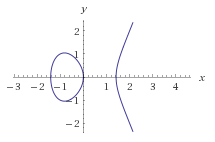
\includegraphics[width=0.5\textwidth]{elliptical}
}\end{center}

\paragraph{(b)}
For the second, we first substitute for $ x $, obtaining $ y^2 = (z + \frac{1}{3})^3 - \frac{4}{3}(z + \frac{1}{3}) - \frac{16}{27} $. This
simplifies to $ y^2 = z^3 + z^2 - z - 1 $. Noticing that one solution to this is $ z = 1 $, we divide:

\polylongdiv[vars=z]{z^3 + z^2 - z - 1}{z - 1}

The resulting quadratic has a single repeated root, $ z = -1 $. Hence, it seems that
we have two solutions for $ z $: $ z = -1 $ and $ z = 1 $. If we take $ z = -1 $ we have $ x = -\frac{2}{3} $,
which gives us $ y^2 = \left(-\frac{2}{3}\right)^3 - \frac{4}{3} \left(-\frac{2}{3}\right) - \frac{16}{27} = 0 $
and so $ z = 1 $ satisfies the original equation; and if we take $ z = 1 $ we have $ x = \frac{4}{3} $ and
$ y^2 = \left(\frac{4}{3}\right)^3 - \frac{4}{3} \left(\frac{4}{3}\right) - \frac{16}{27} = 0 $.

At the time of writing, WolframAlpha only finds a single solution ($ x = -\frac{2}{3}$).

The substitution $ z = x - \frac{b}{3a} $ is a standard one to remove the quadratic term from
a cubic equation $ az^3 + bz^2 + cz + d = 0 $; see exercise \ref{ex:UnpronouncableTransvestite}.

\paragraph{(c)}
Let $ \mathcal{E} $ be the curve $ y^2 = x^3 + ax + c $, and let $ \mathcal{L} $ be the line $ y = mx + c $. Then we wish to
find the solutions to $ (mx + c)^2 = x^3 + ax + b $. Expanding and rearranging, we find that
\begin{displaymath}
  0 = x^3 + m^2 x^2 + (a + 2mc)x + b + c^2.
\end{displaymath}
We know that two solutions to this equation are rational. However, note that $ m^2 $ is the sum of the
three solutions (why?) and is itself rational; hence the third solution must also be rational (and so the two
coordinates of the corresponding point on $ \mathcal{E} $ are rational).

\clearpage
\filbreak\begin{enumerate}[resume]
  \answer The polynomial $ x^3 + px - 1 $ has three real non-zero roots, $ \alpha $,
        $ \beta $, and~$ \gamma $.
        \begin{enumerate}
          \answerb Find the value of $ \alpha^2 + \beta^2 + \gamma^2 $ in terms of $ p $,
                and hence show that $ p $ is negative.
          \answerb Find the cubic polynomial with coefficients in terms of $ p $ with the
                roots $ \alpha^2 $, $ \beta^2 $, and~$ \gamma^2 $.
        \end{enumerate}
\end{enumerate}

\paragraph{(a)}
We first have that $(x - \alpha)(x - \beta)(x - \gamma) = x^3 - (\alpha + \beta + \gamma)x^2 + (\alpha\gamma + \beta\gamma + \alpha\beta)x - \alpha\beta\gamma$.
Matching coefficients, $ 0 = \alpha + \beta + \gamma $ and $ p = \alpha\gamma + \beta\gamma + \alpha\beta $.
Squaring the first: $ (\alpha + \beta + \gamma)^2 = \alpha^2 + \beta^2 + \gamma^2 + 2(\alpha\gamma + \beta\gamma + \alpha\beta) = \alpha^2 + \beta^2 + \gamma^2 + 2p $.
So $ 0 = \alpha^2 + \beta^2 + \gamma^2 + 2p $, and $ -2p = \alpha^2 + \beta^2 + \gamma^2 $. But since the roots are all real and non-zero, $ \alpha^2 + \beta^2 + \gamma^2 > 0 $
and therefore $ p $ must be negative.

\paragraph{(b)}
In order to find the polynomial, we let $ z = x^2 $ and substitute. We have:
\begin{align*}
  x^3 + px &= 1\\
  x(x^2 + p) &= 1\\
  x^2(x^2 + p)^2 &= 1^2 = 1\\
  z(z+p)^2 = 1\\
  z^3 + 2pz^2 + zp^2 - 1 &= 0.
\end{align*}

Alternatively, we can form $ (x - \alpha^2)(x - \beta^2)(x - \gamma^2) $ and then substitute
in the identities $ \alpha^2 + \beta^2 + \gamma^2 = -2p $, $ \alpha^2 \beta^2 \gamma^2 = (\alpha\beta\gamma)^2 = 1 $,
and $ (\alpha^2\beta^2 + \alpha^2\gamma^2 + \beta^2\gamma^2) = (\alpha\beta + \alpha\beta + \beta\gamma)^2 = p^2 $
to find the same polynomial.

\filbreak\begin{enumerate}[resume]
  \answer Take the general cubic, $ at^3 + bt^2 + ct + d $. Show that the substitution $ t = y - \frac{b}{3a} $
        will give a cubic in $ y $ with no quadratic term (this is known as a Tschirnhaus substitution and is
        the first step to create a general formula to solve the cubic). \label{ex:UnpronouncableTransvestite}
\end{enumerate}

We have:
\begin{align*}
  t^2 &= \left( y - \frac{b}{3a} \right)^2\\
      &= y^2 - \frac{2b}{3a}y + \frac{b^2}{9a^2}\\
  t^3 &= \left( y^2 - \frac{2b}{3a}y + \frac{b^2}{9a^2} \right)\left( y - \frac{b}{3a} \right)\\
      &= y^3 - \frac{2b}{3a}y^2 + \frac{b^2}{9a^2}y - \frac{b}{3a}y^2 + \frac{2b^2}{9a^2}y - \frac{b^3}{27a^3}\\
      &= y^3 - \frac{b}{a}y^2 + \frac{b^2}{3a^2}y - \frac{b^3}{27a^3}.
\end{align*}

Substituting, we have
\begin{displaymath}
  a\left(y^3 - \frac{b}{a}y^2 + \frac{b^2}{3a^2}y - \frac{b^3}{27a^3}\right) + b\left(y^2 - \frac{2b}{3a}y + \frac{b^2}{9a^2}\right) + c\left( y - \frac{b}{3a} \right) + d
\end{displaymath}
which we regroup to obtain
\begin{displaymath}
  ay^3 + y^2(-b + b) + y\left( \frac{b^2}{3a} - \frac{2b^2}{3a} + c \right) - \frac{b^3}{27a^2} + \frac{b^3}{9a^2} - \frac{bc}{3a} + d
\end{displaymath}
in which the quadratic term obviously vanishes.

\filbreak\begin{enumerate}[resume]
  \answer Show that $ \sqrt{2} + \sqrt{3} = \sqrt{5 + \sqrt{6}} $.
\end{enumerate}
Note $ \sqrt{5 + \sqrt{6}} = \sqrt{2 + \sqrt{2}\sqrt{3} + 3} = \sqrt{(\sqrt{2} + \sqrt{3})^2} = \abs{\sqrt{2} + \sqrt{3}} $;
but square roots are positive, so $ \abs{\sqrt{2} + \sqrt{3}} = \sqrt{2} + \sqrt{3} $.

\filbreak\begin{enumerate}[resume]
  \answer Prove the following identity.\footnote{~See chapter 1 of Stewart (2004) for historical context,
        but note that the identity as stated there is in error (and not listed in errata).}
        \begin{displaymath}
          \sqrt[3]{-18 + \sqrt{325}} + \sqrt[3]{-18 - \sqrt{325}} = -3
        \end{displaymath}
\end{enumerate}

Let $ u = -18 + \sqrt{325} $ and $ v = -18 - \sqrt{325} $.
In order to prove this identity, we first require the following lemma:
\begin{lemma}
  The two roots of $ p = t^2 + 3t - 1 $ can be expressed as $ \sqrt[3]{u} $
  and $ \sqrt[3]{v} $.
\end{lemma}

Call the two roots of $ p $ $ \alpha $ and $ \beta $. By the quadratic formula,
$ \alpha = \frac{-3 + \sqrt{13}}{2} $. We now show that $ \alpha^3  = u $,
and therefore (since we are working in the reals and so each number has a single
unique cube root) $ \alpha = \sqrt[3]{u} $:
\begin{align*}
  \alpha^3 &= \left( \frac{-3}{2} + \frac{\sqrt{13}}{2} \right)^3\\
           &= -\frac{27}{8} + 3 \cdot \frac{9}{4} \cdot \frac{\sqrt{13}}{2} - 3 \cdot \frac{3}{2} \cdot \frac{13}{4} + \frac{13\sqrt{13}}{8}\\
           &= -\frac{27}{8} + \frac{27\sqrt{13}}{8} - \frac{117}{8} + \frac{13\sqrt{13}}{8}\\
           &= \frac{1}{8}(-144 + 40\sqrt{13})\\
           &= -18 + 5\sqrt{13} = u.
\end{align*}
Likewise, $ \beta = \frac{-3 - \sqrt{13}}{2} = \sqrt[3]{v} $.

\begin{thm}
  That $ \sqrt[3]{-18 + \sqrt{325}} + \sqrt[3]{-18 - \sqrt{325}} = -3 $.
\end{thm}

From the lemma, we have $ p = \left(t - \sqrt[3]{u} \right)\left(t - \sqrt[3]{v} \right) $.
Expanding, $ p = t^2 - \left(\sqrt[3]{u} + \sqrt[3]{v} \right)t + \sqrt[3]{u}\sqrt[3]{v} $,
and matching coefficients with the definition of $ p $ in the lemma we have
$ -3 = \sqrt[3]{u} + \sqrt[3]{v} $.

\filbreak\begin{enumerate}[resume]
  \answer Let $ w = a + b\sqrt{2} + c\sqrt{3} + d\sqrt{6} $, where $ a $, $ b $, $ c $, and $ d $ are rational.
        Find rational numbers $ p $, $ q $, $ r $ and $ s $ such that
        \begin{displaymath}
          w = p + q(\sqrt{2}  + \sqrt{3}) + r(\sqrt{2} + \sqrt{3})^2 + s(\sqrt{2} + \sqrt{3})^3.
        \end{displaymath}
\end{enumerate}

Note that $ (\sqrt{2} + \sqrt{3})^2 = 5 + 2\sqrt{6} $ and $ (\sqrt{2} + \sqrt{3})^3 = 11\sqrt{2} + 9\sqrt{3} $, so we
are trying to find $ p $, $ q $, $ r $, and $ s $ such that
\begin{align*}
  a + b\sqrt{2} + c\sqrt{3} + d\sqrt{6} &= p+ 5r + q\sqrt{2} + q\sqrt{3} + 2r\sqrt{6} + 11s\sqrt{2} + 9s\sqrt{3}\\
                                        &= (p + 5r) + (q + 11s)\sqrt{2} + (q + 9s)\sqrt{3} + 2r \sqrt{6}.
\end{align*}
Hence $ r = d/2 $, $ p = a - 5r = a - \frac{5}{2}d $, $ s = \frac{b - c}{2} $, and $ q = b\left(1 - \frac{11(b-c)}{2}\right) $.

\filbreak\begin{enumerate}[resume]
  \answer Show that there are no integers $ r $ and $ s $ such that $ \sqrt{2} = \frac{r}{s} \sqrt{3} $.
\end{enumerate}
Suppose that such integers exist, and that they are coprime (i.e. $ r/s $ is in lowest form); then we play the familar game. In particular, we note
that $ 3r^2 = 2s^2 $. By Euclid's lemma, $ s $ must be a multiple of $ 3 $; let's write $ s = 3^n p $ for the largest possible $ n $ (so $ p $ is not
a multiple of 3). Substituting back in, we have $ r^2 = \frac{2(3^n p)^2}{3} = 2 \times 3^{2n - 1}p^2 $. But looking at this carefully, we have an odd power
of 3 on the right, and all the prime powers of $ r^2 $ must be even! This is a contradiction, and so there exists no rational number $ r/s $.

\begin{mdframed}[hidealllines=true,backgroundcolor=Emerald!20]
\textit{In particular, we have shown that if we consider $ \mathbb{R} $ a vector space over the rational numbers, then $ \sqrt{2} $ and $ \sqrt{3} $
        are linearly independent. This is a counterexample to the intuitive `theorem' that the real field has no non-identity automorphisms over
        the rationals: simply take the function that swaps $ \sqrt{2} $ and $ \sqrt{3} $!}
\end{mdframed}

\section{Complex Numbers}
% \begin{enumerate}
%   \answer Discuss how the addition and subtraction of complex numbers should be defined.
% \end{enumerate}
%
% Add the real and imaginary parts seperately (i.e. vector addition): $ (a+bi) + (c+di) = (a+b) + (c+d)i $

\begin{enumerate}
  \answer Evaluate the following expressions, and plot the answers on an Argand diagram:
        \begin{enumerate}
          \answerb $ (3+2i) + (6-2i) $
          \answerb $ 24 - (6 + 2i) $
          \answerb $ 2(2+i) + 6i - 7 $
        \end{enumerate}
\end{enumerate}

The three points are 9, $ 22 - 2i $, and $ -3 + 8i $.

\begin{center}\fbox{
\begin{tikzpicture}
  \begin{axis}[
    xlabel=$\realp{z}$,
    ylabel={$\imagp{z}$},
    axis lines=middle
  ]
    \addplot[color=Emerald, mark=o]
    coordinates {
      (9, 0)
    };
    \addplot[color=Emerald, mark=o]
    coordinates {
      (22, -2)
    };
    \addplot[color=Emerald, mark=o]
    coordinates {
      (-3,8)
    };
  \end{axis}
\end{tikzpicture}
}\end{center}

\filbreak\begin{enumerate}[resume]
  \answer If we add two real numbers, can we obtain an imaginary number? If we add two
        imaginary numbers, can we obtain a real number?
\end{enumerate}

If we add two real numbers, we cannot obtain an imaginary number; however, it is possible
to add two imaginary numbers, and obtain zero (a real number). For example, $ -i + i = 0 \in \mathbb{R} $.

\filbreak\begin{enumerate}[resume]
  \answer Let $ v = 3-7i $ and $ w = -4+6i $.
    \begin{enumerate}
      \answerb Find the real numbers $ p $ and $ q $ such that $ pv + qw = 6.5 - 11i $.
      \answerb Show that any complex number $ z $ can be written as $ z = pv + qw $ for some real $ p $ and $ q $.
    \end{enumerate}
\end{enumerate}

\paragraph{(a)}
We have $ p(3 - 7i) + q(-4 + 6i) = (3p -4q) + i(-7p + 6q) $, and so:
\begin{align*}
  3p - 4q &= 6.5\\
  -7p + 6q &= -11
\end{align*}
Hence $ p = \frac{1}{2} $ and $ q = -\frac{5}{4} $.

\paragraph{(b)}
We wish to find $ a $ and $ b $ such that $ 1 = a(3-7i) + b(-4 + 6i) $. This gives us the set of simultaneous equations
\begin{align*}
  1 &= 3a - 4b\\
  0 &= 6b - 7a
\end{align*}
which is easily solved to give $ 1 = -0.6v - 0.7w $. Similarly, $ i = -0.4v - 0.3w $.
Hence if $ z = a + bi $, then $ z = (-0.6v - 0.7w)a + (-0.4v - 0.3w)b = (-0.6a - 0.4b)v + (-0.7a - 0.3b)w $.

\filbreak\begin{enumerate}[resume]
  \answer Solve the quadratic equation $ x^2 + 4 = 0 $.
\end{enumerate}

$ x = \pm 2i $.

\filbreak\begin{enumerate}[resume]
  \answer Prove that $ z + \bar z = 2 \cdot \realp{z} $ and $ z - \bar z = 2i \cdot \imagp{z} $.
\end{enumerate}

Let $ z = x + yi $. Then $ z + \bar z = x + yi + x - yi = 2x = 2\realp{z} $.

Similarly, $ z - \bar z = x + yi -x + yi = 2yi = 2i\imagp{z} $.

\filbreak\begin{enumerate}[resume]
  \answer Verify the following properties of conjugation.
    \begin{enumerate}
      \answerb $ \bar {\bar z} = z $
      \answerb $ \bar w + \bar z = \overline{w + z} $
      \answerb $ \bar w \bar z = \overline{wz} $
    \end{enumerate}
\end{enumerate}
Suppose $ w = a + bi $ and $ z = c + di $.
\paragraph{(a)}
\begin{displaymath}
  \bar {\bar z} = \overline{c - di} = c + di.
\end{displaymath}

\paragraph{(b)}
\begin{displaymath}
  \bar w + \bar z = a - bi + c - di = (a+c) - (b + d)i = \overline{w + z}.
\end{displaymath}

\paragraph{(c)}
\begin{displaymath}
  \bar w \bar z = (a - bi) (c - di) = (ac - bd) - (bc + ad)i = \overline{(ac - bd) + (bc + ad)i} = \overline{(a + bi)(c + di)} = \overline{wz}.
\end{displaymath}

\filbreak\begin{enumerate}[resume]
  \answer Find $ i^{957} $.
\end{enumerate}
First, note that $ 957 = 956 + 1 = 4(239) + 1 $. So $ i^{957} = i^{4(239 + 1)} = (i^4)^{957} i = 1^{957} i = i $.

\filbreak\begin{enumerate}[resume]
  \answer Show that $ \abs{a + bi} \geq \abs{a} $ and $ \abs{a + bi} \geq \abs{b} $.
\end{enumerate}
We have $ \abs{a + bi} = \sqrt{a^2 + b^2} \geq \sqrt{a^2} = \abs{a} $. Similarly $ \abs{a + bi} = \sqrt{a^2 + b^2} \geq \sqrt{b^2} = \abs{b} $.

\filbreak\begin{enumerate}[resume]
  \answer Find $ (3 + 2i)(6 + 8i) $ in rectangular form.
\end{enumerate}
$ (3 + 2i)(6 + 8i) = 18 + 12i + 24i + 16i^2 = 2 + 36i $.

\filbreak\begin{enumerate}[resume]
  \answer \begin{enumerate}
          \answerb Convert $ 1 + i $ into polar form.
          \answerb Find $ (1 + i)(\sqrt{2} \cis \frac{3\pi}{4}) $ in both polar form and rectangular form.
        \end{enumerate}
\end{enumerate}
\paragraph{(a)}
We have $ 1 + i = \sqrt{2} \cis \frac{\pi}{4} $.

\paragraph{(b)}
\begin{align*}
  (1 + i)(\sqrt{2} \cis \frac{3\pi}{4}) &= (\sqrt{2} \cis \frac{\pi}{4})(\sqrt{2} \cis \frac{3\pi}{4})\\
                                        &= 2 \cis \pi
                                        &= -2.
\end{align*}

\filbreak\begin{enumerate}[resume]
  \answer Compute $ (6 \cis \frac{23\pi}{24})(9\cis \frac{14\pi}{17}) $, leaving your answer in polar form.
\end{enumerate}
\begin{displaymath}
  54 \cis \left(\frac{23\pi}{24} + \frac{14\pi}{17}\right) = 54 \cis \frac{727\pi}{408}.
\end{displaymath}

\filbreak\begin{enumerate}[resume]
  \answer \begin{enumerate}
          \answerb Prove that $ (r \cis \theta)(t \cis \varphi) = (rt) \cis (\theta + \varphi) $.
          \answerb Describe the geometric meaning of the multiplication of complex numbers.
        \end{enumerate}
        \label{qn:Moivre1}
\end{enumerate}
\paragraph{(a)}
\textbf{Trigonometric Proof:}
\begin{align*}
  (r \cis \theta)(t \cis \varphi) &= r(\cos \theta + i\sin \theta) \times t(\cos \varphi + i\sin \varphi)\\
                                  &= rt((\cos \theta)(\cos \varphi) - (\sin\theta)(\sin\varphi) + i(\sin\theta\cos\varphi + \cos\theta\sin\varphi))\\
                                  &= rt(\cos(\theta + \varphi) + i(\sin(\theta + \varphi)))\\
                                  &= rt \cis(\theta + \varphi).
\end{align*}

\textbf{Analytic Proof:}
\begin{align*}
  (r \cis \theta)(t \cis \varphi) &= re^{i\theta} \cdot te^{i\varphi}\\
                                  &= rte^{i\theta + i\varphi}\\
                                  &= rte^{i(\theta + \varphi)}\\
                                  &= rt \cis(\theta + \varphi).
\end{align*}

\paragraph{(b)}
The act of complex multiplication both scales the point (by a factor of the modulus) and rotates it around the origin (by the argument).

\filbreak\begin{enumerate}[resume]
  \answer Let $ u = 2 \cis \frac{\pi}{2} $ and $ v = 3 cis \frac{3\pi}{2} $. Plot $ u $, $ v $, and $ uv $ on an Argand diagram.
\end{enumerate}

$ uv = 6 \cis 2\pi = 6 $.

\begin{center}\fbox{
\begin{tikzpicture}
  \begin{axis}[
    xlabel=$\realp{z}$,
    ylabel={$\imagp{z}$},
    axis lines=middle
  ]
    \addplot[color=Emerald, mark=o]
    coordinates {
      (6, 0) % uv
    };
    \addplot[color=Emerald, mark=o]
    coordinates {
      (0, 2) % u
    };
    \addplot[color=Emerald, mark=o]
    coordinates {
      (0,-3) % v
    };
  \end{axis}
\end{tikzpicture}
}\end{center}

\filbreak\begin{enumerate}[resume]
  \answer Prove \textbf{de Moivre's Theorem}: $ (r \cis \theta)^n = (r^n) \cis (n\theta) $.
\end{enumerate}

\textbf{Trigonometric Proof:}
Induction on $ n $ using the result in \ref{qn:Moivre1}.

\textbf{Analytic Proof:}
\begin{align*}
  (r \cis \theta)^n &= \left(re^{i\theta}\right)^n\\
                    &= r^n \left(e^{i\theta}\right)^n\\
                    &= r^n e^{in\theta}\\
                    &= (r^n) \cis (n\theta).
\end{align*}

\filbreak\begin{enumerate}[resume]
  \answer Show that if $ u = r \cis \theta $ and $ v = t \cis \varphi $ then $ \frac{u}{v} = \frac{r}{t}\cis(\theta - \varphi) $.
\end{enumerate}

Taking $ (t \cis \varphi)^{-1} $, we obtain $ \frac{1}{t} \cis (-\varphi) $ (using de Moivre's Theorem), and so
\begin{displaymath}
  \frac{r \cis \theta}{t \cis \varphi} = \frac{r}{t} \cis (\theta - \varphi).
\end{displaymath}

\filbreak\begin{enumerate}[resume]
  \answer Using de Moirve's Theorem, prove that for complex numbers $ w $ and $ m $ and integers $ n $ and $ m $,
    \begin{enumerate}
      \answerb $ w^n w^m = w^{n + m} $
      \answerb $ (w^n)^m = w^{nm} $
    \end{enumerate}
\end{enumerate}
Let $ w = r \cis \theta $.
\paragraph{(a)}
$ w^n w^m = r^n \cis n\theta r^m \cis m\theta = r^{n + m} \cis (n + m)\theta = w^{n + m} $

\paragraph{(b)}
$ (w^n)^m = (r^n \cis n\theta)^m = (r^n)^m \cis nm\theta = r^{nm} \cis nm\theta = w^{nm} $.

\filbreak\begin{enumerate}[resume]
  \answer Convert $ w = 1 + \sqrt{3}i $ into polar form, and calculate $ w^3 $.
\end{enumerate}

$ \abs{w} = \sqrt{1^2 + \sqrt{3}^2} = 2 $, $ \carg{w} = \arctan{\frac{\sqrt{3}}{1}} = \frac{\pi}{3} $.

Hence $ w^3 = (2 \cis \frac{\pi}{3})^3 = 2^3 \cis \pi = -8 $, using de Moivre's Theorem.

\filbreak\begin{enumerate}[resume]
  \answer Show that for any complex number $ z $, the product $ z \bar z $ is both real and non-negative.
        Hence show that $ (x - z)(x - \bar z) $ has only real coeffients. \label{qn:rationalise}
\end{enumerate}

Let $ z = a + bi $. Then $ z \bar z = (a+bi)(a-bi) = a^2 + b^2 $, which is real and positive (or zero). This
also provides an identity for the sum of two squares.

$ (x - z)(x - \bar z) = x^2 - (z + \bar z) + z \bar z = x^2 + 2a + a^2 + b^2 $, and since $ a,b \in \mathbb{R} $
the coefficients are real.

\filbreak\begin{enumerate}[resume]
  \answer Let $ x $ be a real number. Show that, for all integers $ n $, $ \cis \frac{2x\pi}{n} = \cis \frac{2(x + n)\pi}{n} $.
\end{enumerate}
We argue as follows:
\begin{align*}
  \cis \frac{2(x + n)\pi}{n} &= \cos \frac{2(x + n)\pi}{n} + i\sin \frac{2(x + n)\pi}{n}\\
                             &= \cos \frac{2x\pi}{n} \cos{2\pi} - \sin\frac{2x\pi}{n} \sin{2\pi} + i(\sin\frac{2x\pi}{n} \cos{2\pi} + \cos\frac{2x\pi}{n} \sin{2\pi})\\
                             &= \cos \frac{2x\pi}{n} \cdot 1 - \sin\frac{2x\pi}{n} \cdot 0 + i(\sin\frac{2x\pi}{n} \cdot 1 + \cos\frac{2x\pi}{n} \cdot 0)\\
                             &= \cos \frac{2x\pi}{n} + i\sin \frac{2x\pi}{n}\\
                             &= \cis \frac{2x\pi}{n}.
\end{align*}

\filbreak\begin{enumerate}[resume]
  \answer For which complex numbers is $ z^2 $ real? What about $ z^3 $?
\end{enumerate}

Let $ z = x + yi $. Then $ z^2 = x^2 + 2xyi - y^2 $, which will be real if and only
if $ 2xy = 0 $; so at least one of $ x $ or $ y $ must be zero for $ z $ to be real.
In other words, $ z $ must be either totally real or totally imaginary.

For the cube, we have $ z^3 = x^3 + 3x^2yi - 3xy^2 - iy^3 $. For $ z^3 $ to be real,
we must have $ 3x^2y - y^3 = 0 $. This will occur when $ y = 0 $; noting this, we suppose
$ y \neq 0 $ and divide through by $ y $, obtaining $ 3x^2 = y^2 $. Solving this, we find
$ y = \pm \sqrt{3} x $. So $ z^3 $ will be real either if $ z $ is totally real, or if
$ \imagp{z} = \pm\sqrt{3} \realp{z} $.

\filbreak\begin{enumerate}[resume]
  \answer Transform $ \frac{a+bi}{c+di} $ so that the only imaginary part is in the numerator.
\end{enumerate}

Using the idea from question \ref{qn:rationalise}:

$ \frac{a+bi}{c+di} = \frac{(a+bi)(c-di)}{(c+di)(c-di)} = \frac{ac + bd + (bc - ad)i}{c^2 + d^2} $,
where the denominator is real.

\filbreak\begin{enumerate}[resume]
  \answer Find $ (a+bi)^{-1} $.
\end{enumerate}
\begin{align*}
  \frac{1}{a+bi} &= \frac{a-bi}{(a+bi)(a-bi)}\\
                 &= \frac{a-bi}{a^2 + b^2}\\
                 &= \frac{a}{a^2 + b^2} - \frac{b}{a^2 + b^2}i.
\end{align*}

\filbreak\begin{enumerate}[resume]
  \answer Write the complex number $ \left( \frac{4i^7 - i}{1+2i} \right)^2 $ in the
        form $ a + bi $, where $ a $ and $ b $ are real numbers.
\end{enumerate}
\begin{align*}
  \left( \frac{4i^7 - i}{1+2i} \right)^2 &= \left( \frac{-4i - i}{1+2i} \right)^2\\
                                         &= \left( \frac{-5i}{1+2i} \right)^2\\
                                         &= \frac{25}{-3+4i}\\
                                         &= \frac{25(-3-4i)}{(-3+4i)(-3-4i)}\\
                                         &= \frac{25{-3-4i}}{25}\\
                                         &= -3-4i.
\end{align*}

\filbreak\begin{enumerate}[resume]
  \answer
    \begin{enumerate}
      \answerb Prove that a number $ z $ is real if and only if $ \bar z = z $.
      \answerb Hence, or otherwise, show that $ z \bar w + w \bar z $ is always real.
      \answerb Show that $ z \bar w + w \bar z \leq 2 \abs{w} \abs{z} $.
    \end{enumerate}
\end{enumerate}
\paragraph{(a)}
Let $ z = a + bi $. Suppose $ z $ is real. Then $ b = 0 $, and $ \bar z = \overline{a + 0i} = a - 0i = z $.
Conversely, suppose $ \bar z = z $. Then $ a - bi = a + bi $, and $ b = -b $; hence $ b = 0 $ and $ z $ is real.

\paragraph{(b)}
By part (a), we need only check that the given expression is its own conjugate:
\begin{displaymath}
  \overline{z \bar w + w \bar z} = \overline{z \bar w} + \overline{w \bar z} = \bar z \bar {\bar w} + \bar w \bar {\bar z} = \bar z w + \bar w z
\end{displaymath}

\paragraph{(c)}
Let $ z = r \cis \theta $ and $ w = t \cis \phi $. Then we have:
\begin{align*}
  z \bar w + w \bar z &= (r \cis \theta)(t \cis -\phi) + (t \cis \phi)(r \cis -\theta)\\
                      &= (rt) \cis (\theta - \phi) + (rt) \cis(\phi - \theta)\\
                      &= rt(\cos (\theta - \phi) + \cos(\phi - \theta) + i(\sin(\theta - \phi) + \sin(\phi - \theta)))\\
                      &= 2rt\cos(\theta - \phi)\\
                      &\leq 2rt \quad\quad \text{(since $ \cos x \leq 1 $)}\\
                      &= 2 \abs{z} \abs{w}.
\end{align*}

\filbreak\begin{enumerate}[resume]
  \answer Show that if $ z = a + ib $ then $ \sqrt{z\bar z} = \abs{z} $.
\end{enumerate}
From question \ref{qn:rationalise}, we have $ z\bar z = a^2 + b^2 $; hence $ \sqrt{z\bar z} = \sqrt{a^2 + b^2} = \abs{z} $.

\filbreak\begin{enumerate}[resume]
  \answer If $ \zeta = \sqrt{\frac{1}{2}(a+\sqrt{a^2+b^2})} + i\sqrt{\frac{1}{2}(-a+\sqrt{a^2+b^2})} $
        is a complex number, find $ \zeta^2 $ in the form $ p + iq $ (where $ a $, $ b $, $ p $, and $ q $ are real).
\end{enumerate}
\begin{align*}
  &\left( \sqrt{\frac{1}{2}(a+\sqrt{a^2+b^2})} + i\sqrt{\frac{1}{2}(-a+\sqrt{a^2+b^2})} \right)^2\\
  &= \frac{1}{2}(a+\sqrt{a^2+b^2}) + 2i\sqrt{\frac{1}{2}(a+\sqrt{a^2+b^2)})}\sqrt{\frac{1}{2}(-a+\sqrt{a^2+b^2)})} - \frac{1}{2}(-a+\sqrt{a^2+b^2})\\
  &= a + 2i\sqrt{\frac{1}{4}(\sqrt{a^2+b^2} + a)(\sqrt{a^2+b^2} - a)}\\
  &= a + 2i\sqrt{\frac{1}{4}((a^2+b^2)-a^2)}\\
  &= a + 2i\sqrt{\frac{b^2}{4}}\\
  &= a+bi.
\end{align*}

\filbreak\begin{enumerate}[resume]
  \answer If $ z = x + iy $, and $ az^2 + bz + c = 0 $, show that $ a \overline z^2 + b \overline z + c = 0 $
        if $ a $, $ b $, and $ c $ are real. (This exercise is generalised in 9.\ref{ex:solutiongenerator}.) \label{ex:conjquadratic}
\end{enumerate}

See the exercise noted in the question for an easier way to prove this (which requires a bit less work).

Let the value of $ a \bar z^2 + b \bar z + c $ be $ K $ --- our goal is to prove that $ K = 0 $.

We have that
\begin{align*}
  a \bar z^2 + b \bar z + c &= a(x-iy)^2 + b(x-iy) + c\\
                            &= ax^2 - 2aixy - ay^2 + bx - biy + c = K. \tag{1}
\end{align*}
And that
\begin{align*}
  a z^2 + b z + c &= a(x+iy)^2 + b(x+iy) + c\\
                  &= ax^2 + 2aixy - ay^2 + bx + biy + c = 0. \tag{2}
\end{align*}
Note that the real part of this equation is $ ax^2 - ay^2 + bx + c $.

Since the second equation is equal to zero, we can add it to the first:
\begin{align*}
   &(&& ax^2 &&- 2aixy &&- ay^2 &&+ bx &&- biy &&+ c &&= K) \tag{1}\\
  +&(&& ax^2 &&+ 2aixy &&- ay^2 &&+ bx &&+ biy &&+ c &&= 0) \tag{2}\\
  =& &&2ax^2 &&        &&-2ay^2 &&+2bx &&      &&+2c &&= K) \tag{3}
\end{align*}
But we notice that the real part of (2) must be equal to zero --- and equation
(3) is simply twice the real part of (2), so $ K = 0 $.

\filbreak\begin{enumerate}[resume]
  \answer Use Euler's identity to find $ \ln (-1) $, and hence $ \ln (-x) $ for real $ x $.
\end{enumerate}
\begin{align*}
  e^{i\pi} &= -1\\
  i\pi     &= \ln{(-1)}\\
\end{align*}
Notice that $ \cis \theta = e^{i\pi} $ is has a period of $ 2\pi $,
so $ \ln{(-1)} = i(\pi + 2n\pi) $ for $ n\in\mathbb{N} $.
\begin{align*}
  \ln{-x} &= \ln{(-1 \times x)}\\
          &= \ln{(-1)} + \ln{x}\\
          &= \ln{x} + i\pi(1+2n).
\end{align*}

\filbreak\begin{enumerate}[resume]
  \answer Prove that for every positive integer $ n $, $ (-1 + \sqrt{3}i)^{3n} + (-1 - \sqrt{3}i)^{3n} = 2^{3n+1} $.
\end{enumerate}

If we convert $ -1 + \sqrt{3}i $ to polar form, we obtain $ 2 \cis \frac{5\pi}{6} $. Substituting:
\begin{align*}
  (-1 + \sqrt{3}i)^{3n} + (-1 - \sqrt{3}i)^{3n} &= \left(2 \cis \frac{2\pi}{3}\right)^{3n} + \left(2 \cis \frac{-2\pi}{3}\right)^{3n} \\
                                                &= 2^{3n} (\cis 2\pi n) + 2^{3n} \cis (-2 \pi n) \\
                                                &= 2^{3n} + 2^{3n} \\
                                                &= 2^{3n + 1}.
\end{align*}

\filbreak\begin{enumerate}[resume]
  \answer Show that $ y_1(x) = e^{ix} + e^{-ix} $ and $ y_2(x) = 2\cos x $ are both solutions of the differential equation
        \begin{displaymath}
          \od[2]{y}{x} + y = 0
        \end{displaymath}
        with initial conditions $ y(0) = 2 $ and $ y'(0) = 0 $. (Also see \ref{ex:eulersin} below.)
\end{enumerate}

Note that $ y_1'(x) = ie^{ix} - ie^{-ix} $ and $ y_1''(x) = -e^{ix} - e^{-ix} = -y_1 $, so $ y_1 $ is a solution of the differential
equation. We also have $ y_2'(x) = -2\sin x $ and $ y_2'' = -2\cos x = -y_2 $, so $ y_2 $ is also a solution.

We check that the initial conditions hold: $ y_1(0) = 1 + 1 = 2 $ and $ y_1'(0) = i - i = 0 $, and $ y_2(0) = 2 $ and $ y_2'(0) = 0 $
as required. Hence $ y_1 $ and $ y_2 $ are both solutions of the differential equation that satisfy the initial conditions.

Note that in exercise \ref{ex:eulersin} below, it is proved that in fact $ y_1 = y_2 $.

\filbreak\begin{enumerate}[resume]
  \answer Find $ \sqrt{i} $ in rectangular form.
\end{enumerate}
Note that $ i = \cis \frac{\pi}{2} $, so $ \sqrt{i} = \cis (\frac{\pi}{4} + \frac{2n\pi}{2}) $ for $ n \in \{0, 1\} $.
Hence the two square roots are $ \cis \frac{\pi}{4} = \frac{1}{\sqrt{2}} + i\frac{1}{\sqrt{2}} $
and $ \cis \frac{5\pi}{4} = -\frac{1}{\sqrt{2}} - i\frac{1}{\sqrt{2}} $.

\filbreak\begin{enumerate}[resume]
  \answer\label{ex:eulersin}
    \begin{enumerate}
      \answerb Show that $ \cos \theta = \frac{e^{i\theta} + e^{-i\theta}}{2} $ and that $ \sin \theta = \frac{e^{i\theta} - e^{-i\theta}}{2i} $.
      \answerb If $ x + x^{-1} = 2 \cos \theta $, find $ x^n + x^{-n} $ in terms of $ n $ and $ \theta $.
    \end{enumerate}
\end{enumerate}

\paragraph{(a)}
\begin{align*}
  e^{i\theta} + e^{-i\theta} &= \cis \theta + \cis -\theta\\
                             &= \cos \theta + i\sin\theta + \cos -\theta + \sin -\theta\\
                             &= \cos \theta + i\sin\theta + \cos \theta - \sin \theta\\
                             &= 2\cos\theta.\\
  e^{i\theta} - e^{-i\theta} &= \cis \theta - \cis -\theta\\
                             &= \cos \theta + i\sin\theta - \cos -\theta - \sin -\theta\\
                             &= \cos \theta + i\sin\theta - \cos \theta + \sin \theta\\
                             &= 2i\sin\theta.
\end{align*}

\paragraph{(b)}
From (a), $ 2\cos\theta = e^{i\theta} + e^{-i\theta} = e^{i\theta} + \left(e^{i\theta}\right)^{-1} $,
and so $ x = e^{i\theta} $. Hence $ x^n = e^{ni\theta} $, and:
\begin{align*}
  x^n + x^{-n} &= e^{ni\theta} + e^{-ni\theta}\\
               &= \cos n\theta + i\sin n\theta + \cos n\theta - i\sin n\theta\\
               &= 2\cos n\theta.
\end{align*}

\filbreak\begin{enumerate}[resume]
  \answer
    \label{ex:cardano}
    \begin{enumerate}
      \answerb Show that $ (2 \pm i)^3 = 2 \pm 11i $.
      \answerb Simplify fully $ \sqrt[3]{2+\sqrt{-121}} + \sqrt[3]{2-\sqrt{-121}} $.
      \answerb Show that (b) is a root of the cubic equation $ t^3 - 15t - 4 = 0 $,
            and hence find all three solutions.
    \end{enumerate}
\end{enumerate}

Firstly, $ (2 + i)(2 + i)(2 + i) = (3 + 4i)(2 + i) = 2 + 11i $; likewise, we have
$ (2 - i)^3 = 2 - 11i $. Using this result,
we can simplify the expression in (b):
\begin{align*}
  \sqrt[3]{2+\sqrt{-121}} + \sqrt[3]{2-\sqrt{-121}} &= \sqrt[3]{2 + 11i} + \sqrt[3]{2 - 11i}\\
                                                    &= \sqrt[3]{(2 + i)^3} + \sqrt[3]{(2 - i)^3}
                                                    &= (2 + i) + (2 - i)\\
                                                    &= 4.
\end{align*}

It is easy to show that 4 is a root of the cubic in (c): $ 4^3 - 15\cdot4 - 4 = 0 $,
as expected.

We divide the cubic by $ t - 4 $ to reduce it to a quadratic:
\polylongdiv[vars=t]{t^3 - 15t - 4}{t - 4}

By the quadratic formula, the two solutions of the quadratic factor are $ t = -2 \pm \sqrt{3} $,
so the three solutions of the cubic must be $ t \in \{-2\pm\sqrt{3}, 4\} $.

\filbreak\begin{enumerate}[resume]
  \answer You do not need the fundamental theorem of algebra for this exercise.
    \begin{enumerate}
      \answerb Prove that all cubic equations with real coefficients must have exactly three roots in the complex numbers.
      \answerb Let $ p(x) $ be a polynomial of degree $ n $ such that there exists some complex number $ \zeta $ such that $ p(\zeta) = 0 $.
               Show that $ p(x) = 0 $ has exactly $ n $ solutions (counting repeated roots).
    \end{enumerate}
\end{enumerate}

\paragraph{(a)}
A cubic with real coefficients must have at least one real root. There are two ways to see this;
firstly, a cubic with real coefficients must cross the $ x$-axis at at least one point; and secondly,
all non-real roots of polynomials with real coefficients must come in conjugate pairs (in order for the
imaginary parts to cancel in the coefficients) and so a real polynomial with an odd number of roots
must have at least one real root.\footnote{A proof that roots of real polynomials come in conjugate
pairs is exercise 9.\ref{ex:solutiongenerator}.}

Call our real root $ p $. Our cubic is $ a x^3 + b x^2 + cx + d = 0 $, and
we can divide it out by $ x - p $, which we know is a factor, to obtain a
quadratic. We know that the coefficients of this quadratic factor must multiply
with the real coefficients of the linear factor to give the real coefficients of
the cubic, and so the coefficients of the quadratic must be real... and so we can
apply the quadratic formula to show that the roots of the quadratic must be complex!

Hence all three roots of the general cubic are complex. \textit{Note that all real roots
are also complex.}

\paragraph{(b)}
We use induction on $ n $. Firstly, note that if $ n = 1 $ then the result is trivial.

Now, suppose that the theorem holds for all polynomials of degree $ n - 1 $. It follows from $ p(\zeta) = 0 $
that $ (x - \zeta) $ is a factor of $ p(x) $, and so $ p(x) = (x - \zeta)q(x) $ where $ \partial q = n - 1 $.
But by the inductive hypothesis, $ q(x) $ has exactly $ n - 1 $ roots; so $ p(x) $ has $ n $ roots, and if
the theorem holds for polynomials of degree $ n - 1 $ then it holds for polynomials of degree $ n $.

Hence, by the axiom of induction, it follows that if a polynomial of degree $ n $ has at least one complex
root then it has exactly $ n $ complex roots.

\section{Geometry}

\filbreak\begin{enumerate}
  \answer Show that, if $ a $ and $ b $ are fixed complex numbers, then $ \abs{z - a} = \abs{z - b} $ describes the line which
        cuts the midpoint of the segment between $ a $ and $ b $ at a right angle.
\end{enumerate}

Suppose that the distance from $ z $ to $ a $ is equal to the distance from $ z $ to $ b $.

The line joining $ a $ and $ b $ has direction $ a - b $; the line joining $ z $ and $ m(a,b) = \frac{a + b}{2} $ has direction $ z - \frac{a + b}{2} $. I
claim that the two complex numbers obtained are orthogonal. Indeed,
\begin{align*}
  (z - \frac{a + b}{2}, a - b) &= (z, a) - (z, b) - (\frac{a + b}{2}, a) + (\frac{a + b}{2}, b)\\
                               &= (z, a) - (z,b) - \frac{1}{2}((a,a) + (b,a)) + \frac{1}{2}((a,b) + (b,b))\\
                               &= (z,a) - (z,b) + \frac{1}{2}(b,b) - \frac{1}{2}(a,a).
\end{align*}
But $ \abs{z - a} = \abs{z - b} $, so
\begin{displaymath}
  (z - a, z - a) = (z - b, z - b) \implies (z, z) - 2(a,z) + (a,a) = (z,z) - 2(z,b) + (b,b)
\end{displaymath}
and thus $ (z,a) - (z,b) = \frac{1}{2}(a,a) - \frac{1}{2}(b,b) $;
so $ (z - \frac{a + b}{2}, a - b) = 0 $, and the two vectors are orthogonal. So every such $ z $ lies on the perpendicular
bisector of the segment $ [ab] $; and clearly every $ z $ on that line is an equal distance from $ a $ and $ b $.

\filbreak\begin{enumerate}[resume]
  \answer Let $ v = 1 + i $ and $ z = x + iy $ for any real numbers $ x $ and $ y $.
    \begin{enumerate}
      \answerb Show that the equation $ \abs{z - v} = \abs{vz} $ represents a circle, and find its
            centre and radius.
      \answerb Find the point of intersection of the circle with the straight line $ \abs{z - v} = \abs{z + v} $.
    \end{enumerate}
\end{enumerate}

\paragraph{(a)}
Expanding using the distance formula, we have
\begin{align*}
  \abs{z - v} &= \sqrt{(x - 1)^2 + (y - 1)^2} \\
  \abs{vz}    &= \abs{(1 + i)(x + iy)} \\
              &= \abs{x + iy + ix - y} \\
              &= \sqrt{(x - y)^2 + (x+y)^2} \\
              &= \sqrt{2x^2 + 2y^2}\\
              &\Downarrow \\
  (x - 1)^2 + (y - 1)^2 &= 2x^2 + 2y^2 \\
              &\Downarrow  \\
  0           &= x^2 + y^2 + 2x + 2y - 2 \\
              &= (x+1)^2 + (y+1)^2 - 4 \text{ (completing the square)}.
\end{align*}
Hence we have a circle centred on $ (-1, -1) $ with a radius of 2.

\paragraph{(b)}
\begin{center}\fbox{
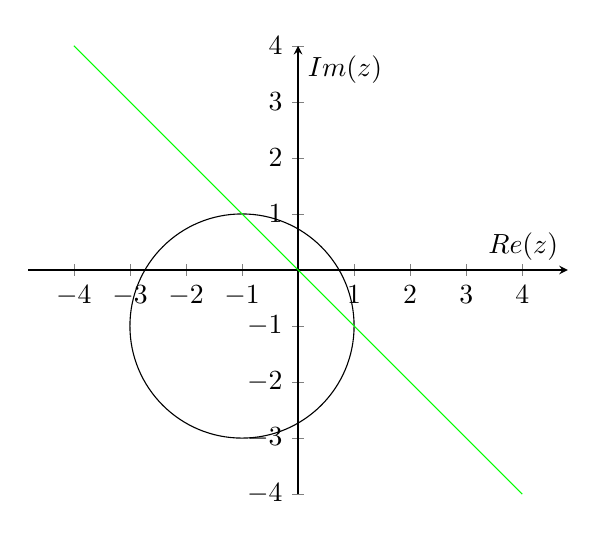
\begin{tikzpicture}
  \begin{axis}[
    xlabel=$Re(z)$,
    ylabel={$Im(z)$},
    axis lines=middle,
     disabledatascaling,
    xmin=-4,
    xmax=4,
    ymin=-4,
    ymax=4,
    xtick={-4, -3, ..., 4},
    ytick={-4, -3, ..., 4},
    axis equal
  ]
  \path [draw=black, fill=none] (-1,-1) circle (2);
  \addplot[domain=-4:4, samples=2, color=green]{-x};
  \end{axis}
\end{tikzpicture}
}\end{center}
Finding the equation of the line:
\begin{align*}
  (x - 1)^2 + (y - 1)^2 &= (x + 1)^2  + (y + 1)^2 \\
  0 &= 4x + 4y \\
  y = -x.
\end{align*}
Substituting:
\begin{align*}
  4 &= (x+1)^2 + (1-x)^2\\
  1 &= x^2\\
  x &= \pm 1\\
  \implies y &= \mp 1
\end{align*}

So the line intersects the circle at $ (-1, 1) $ and $ (1, -1) $.

\filbreak\begin{enumerate}[resume]
  \answer Find the locus of all $ z $ such that for some fixed $ a $, $ z - a $ is perpendicular to $ z + a $.
\end{enumerate}

We have $ (z - a, z + a) = 0 $; so $ (z,z) - (a,z) + (z,a) - (a,a) = 0 $
and thus $ (z,z) = (a,a) $. So $ \sqrt{\abs{z}} = \sqrt{\abs(a)} $, and (since
lengths are positive) $ \abs{z} = \abs{a} $. In other words, we have a circle
around zero of radius $ \abs{a} $.

\filbreak\begin{enumerate}[resume]
  \answer Show that if $ u $, $ v $, and $ w $ are complex numbers, and if $ \lambda $ and $ \mu $ are real
        numbers, then:
    \begin{enumerate}
      \answerb $ (u, v) = (v, u) $
      \answerb $ (\lambda u + \mu v, w) = \lambda(u, w) + \mu(v, w) $
    \end{enumerate}
\end{enumerate}

\paragraph{(a)}
$ (u,v) = \realp{u}\realp{v} + \imagp{u} \imagp{v} = \realp{v}\realp{u} + \imagp{v} \imagp{u} = (v,u) $.

\paragraph{(b)}
\begin{align*}
  (\lambda u + \mu v, w) &= \realp{\lambda u + \mu v} \realp{w} + \imagp{\lambda u + \mu v} \imagp{w}\\
   &= (\lambda \realp{u} + \mu \realp{v}) \realp{w} + (\lambda \imagp{u} + \mu \imagp{v}) \imagp{w}\\
   &= \lambda \realp{u} \realp{w} + \mu \realp{v} \realp{w} + \lambda \imagp{u} \imagp{w} + \mu \imagp{v} \imagp{w}\\
   &= \lambda (\realp{u} \realp{w} + \imagp{u} \imagp{w}) + \mu(\realp{v} \realp{w} + \imagp{v} \imagp{w})\\
   &= \lambda(u, w) + \mu(v, w).
\end{align*}

\section{Roots of Unity}
\begin{mdframed}[hidealllines=true,backgroundcolor=Emerald!20]
\textit{Many of the results here follow from basic results in number theory. The interested reader is directed
        towards `Elementary Number Theory' by Underwood Dudley~\cite{Dud08}. More generally, the material in this chapter
        develops the theory of finite cyclic groups (the $ n$th roots of unity under multiplication form a group isomorphic to
        the finite cyclic group of order $ n $).}
\end{mdframed}

\begin{enumerate}
  \answer Let $ p(z) = z^5 - 1 $.
    \begin{enumerate}
      \answerb Find exactly each of the roots of $ p(z) $.
      \answerb Let $ \alpha $ be the root of $ p $ with the smallest non-zero
            positive argument. Show explicitly that the roots can be written as 1, $ \alpha $,
            $ \alpha^2 $, $ \alpha^3 $, and $ \alpha^4 $.
    \end{enumerate}
\end{enumerate}

\paragraph{(a)}
The five roots will be symmetrical around the $ x$-axis with angles of $ \frac{2\pi}{5} $ separating them:
\begin{center}
\begin{tabular} {c | c}
  \textbf{Root} & \textbf{Polar form}\\
  $ z_0 $ & $ \cis 0 $               \\
  $ z_1 $ & $ \cis \frac{2\pi}{5} $  \\
  $ z_2 $ & $ \cis \frac{-2\pi}{5} $ \\
  $ z_3 $ & $ \cis \frac{4\pi}{5} $  \\
  $ z_4 $ & $ \cis \frac{-4\pi}{5} $
\end{tabular}
\end{center}

\paragraph{(b)}
In this case, we use de Moivre's Theorem:\\
$ z_0 = \alpha^0 = \cis 0\times\frac{2\pi}{5} = 1 $;\\
$ z_1 = \alpha^1 = \cis 1\times\frac{2\pi}{5} = \cis \frac{2\pi}{5} $;\\
$ z_2 = \alpha^4 = \cis 4\times\frac{2\pi}{5} = \cis \frac{8\pi}{5} = \cis \frac{-2\pi}{5} $;\\
$ z_3 = \alpha^2 = \cis 2\times\frac{2\pi}{5} = \cis \frac{4\pi}{5} = \cis \frac{4\pi}{5} $; and\\
$ z_4 = \alpha^3 = \cis 3\times\frac{2\pi}{5} = \cis \frac{6\pi}{5} = \cis \frac{-4\pi}{5} $.

We could also use the result in exercise \ref{ex:smallprimitive} (since $ z_1 = \alpha $ is the 5th root of unity with smallest positive
argument, it is primitive and so generates all the 5th roots of unity).

\filbreak\begin{enumerate}[resume]
  \answer Find all solutions of $ z^3 + n = 0 $, where $ n $ is a positive real number,
        in exact form in terms of $ n $.
\end{enumerate}
Note that $ n = n \cis 0 $ and so $ -n = n \cis \pi $.
\begin{align*}
  z^3 &= -n\\
  z   &= n^{\frac{1}{3}} \cis \left(\pi + \frac{2n\pi}{3}\right)\\
      &= \sqrt[3]{n} \cis \left(\pi + \frac{2n\pi}{3} \right)    &\text{($0 \leq n < 3$)}
\end{align*}
So $ z_0 = \sqrt[3]{n} \cis \pi $, $ z_1 = \sqrt[3]{n} \cis \frac{5\pi}{3} $, $ z_2 = \sqrt[3]{n} \cis \frac{\pi}{3} $ are
the three roots.

\filbreak\begin{enumerate}[resume]
  \answer Solve for $ z $ if $ (z-3)^7 = 1 $.
\end{enumerate}
\begin{center}
\begin{tabular} {c | c}
  \textbf{Root} & \textbf{Polar form}\\
  $ z_0 - 3 $ & $ \cis 0 $               \\
  $ z_1 - 3 $ & $ \cis \frac{2\pi}{7} $  \\
  $ z_2 - 3 $ & $ \cis \frac{-2\pi}{7} $ \\
  $ z_3 - 3 $ & $ \cis \frac{4\pi}{7} $  \\
  $ z_4 - 3 $ & $ \cis \frac{-4\pi}{7} $ \\
  $ z_5 - 3 $ & $ \cis \frac{6\pi}{7} $  \\
  $ z_6 - 3 $ & $ \cis \frac{-6\pi}{7} $
\end{tabular}
\end{center}

Then simply convert each root to rectangular form and add 3.

\filbreak\begin{enumerate}[resume]
  \answer Find the fifth roots of $ 4 + 4i $ in polar form, and draw them on an Argand
        diagram. Hence find integers $ p $ and $ q $ such that $ (p+qi)^5 = (4+4i) $.
\end{enumerate}

Note that $ 4+4i = 4\sqrt{2} \cis \frac{\pi}{4} $. We therefore compute
$ \sqrt[5]{4\sqrt{2} \cis \frac{\pi}{4}} = \sqrt[10]{32} \cis \left( \frac{\pi}{20} + \frac{2n\pi}{5} \right) $
for $ 0 \leq n < 5 $:
\begin{center}
\begin{tabular} {c | c}
  \textbf{Root} & \textbf{Polar form}  \\
  $ z_1 $ & $ \sqrt{2}\cis \frac{\pi}{20}    $ \\
  $ z_2 $ & $ \sqrt{2}\cis \frac{9\pi}{20}   $ \\
  $ z_3 $ & $ \sqrt{2}\cis \frac{17\pi}{20}  $ \\
  $ z_4 $ & $ \sqrt{2}\cis \frac{5\pi}{4}    $ \\
  $ z_5 $ & $ \sqrt{2}\cis \frac{33\pi}{20}  $
\end{tabular}
\end{center}

\begin{center}\fbox{
\begin{tikzpicture}
  \begin{axis}[
     xlabel=$\realp{z}$,
     ylabel={$\imagp{z}$},
     xlabel near ticks,
     ylabel near ticks,
     axis lines=middle,
     xmin=-1.5,
     xmax=1.5,
     ymin=-1.5,
     ymax=1.5
  ]
    \addplot+[color=black, mark=x, data cs=polarrad, only marks]
    coordinates {
      (pi/20, 1.414) (9*pi/20, 1.414) (17*pi/20, 1.414) (5*pi/4, 1.414) (33*pi/20, 1.414) (pi/20, 1.414)
    };
  \end{axis}
\end{tikzpicture}
}\end{center}

Hence the required integer values are $ p = q = -1 $.

\filbreak\begin{enumerate}[resume]
  \answer Write down all of the primitive sixth roots of unity. What about the primitive fifth roots of unity?
\end{enumerate}

Let $ \alpha = \cis \frac{2\pi}{6} $. Then the sixth roots of unity are:
\begin{center}
\begin{tabular} {c | c}
  \textbf{Root} & \textbf{Polar form}\\
  $ z_0 $ & $ \cis 0 $               \\
  $ z_1 $ & $ \cis \frac{2\pi}{6} = \cis \frac{\pi}{3} $   \\
  $ z_2 $ & $ \cis \frac{4\pi}{6} = \cis \frac{2\pi}{3} $  \\
  $ z_3 $ & $ \cis \frac{6\pi}{6} = \cis \frac{2\pi}{2} $  \\
  $ z_4 $ & $ \cis \frac{8\pi}{6} = \cis \frac{4\pi}{3} $  \\
  $ z_5 $ & $ \cis \frac{10\pi}{6} = \cis \frac{5\pi}{3} $
\end{tabular}
\end{center}

It is clear that $ z_2 $ and $ z_4 $ are third roots of unity, and that $ z_3 $ is a square root of unity. This
just leaves $ z_1 $ and $ z_5 $ as primitive sixth roots of unity.

The primitive fifth roots of unity are all the fifth roots of unity (except 1 itself); more generally, the primitive $ p$th
roots of unity ($ p $ prime) are all the $ p$th roots of unity (again, excluding 1).

\filbreak\begin{enumerate}[resume]
  \answer \label{ex:rootsum}
    \begin{enumerate}
      \answerb Let $ \alpha $ be a complex root of $ x^3 = 1 $. Show by computation that $ \alpha^2 + \alpha + 1 = 0 $.
      \answerb In general, prove that the sum of all $ n $ $ n$th roots of unity is zero (for $ n > 1 $).
    \end{enumerate}
\end{enumerate}

\paragraph{(a)}
We have that $ (x - 1) $ is a root of the polynomial; by long division, $ x^2 + x + 1 $ is the
quadratic factor. Since $ \alpha \neq 1 $, it must be a root of this quadratic; and so
$ \alpha^2 + \alpha + 1 = 0 $.

\polylongdiv{x^3 - 1}{x - 1}

This demonstrates that the sum of all three third roots of unity is zero, and the same technique can be used for (b).

\paragraph{(b)}
Let $ \omega $ be a primitive $ n$th root of unity. Then all the $n$th roots of unity are given by $ \omega^0, \omega^1, \dots, \omega^{n-1} $.
Also note that $ 0 = \omega^n - 1 = (\omega - 1)(1 + \omega + \cdots + \omega^{n - 1}) $. But $ \omega $ is primitive, and so in particular
is not equal to one. So we can divide through by $ (\omega - 1) $ to obtain the required result.

Geometrically, this result can also be seen by drawing a diagram and taking vector sums.

\filbreak\begin{enumerate}[resume]
  \answer Find the product of all $ n $ $n$th roots of unity.
\end{enumerate}
Suppose $ \{\omega_0, \omega_1, \dots, \omega_{n-1}\} $ are the $ n$th roots of unity,
where $ \omega_k = \cis\left( \frac{2k\pi}{n} \right) $. Then:
\begin{align*}
  \prod_{k = 0}^{k < n} \cis\left( \frac{2k\pi}{n} \right) &= \cis \left( \sum_{k = 0}^{k < n} \frac{2k\pi}{n} \right)\\
                                                           &= \cis \left( \frac{2\pi}{n} \cdot \frac{(n-1)n}{2} \right)\\
                                                           &= \cis \left( (n-1)\pi \right)\\
                                                           &= \cos \left( (n-1)\pi \right)\\
                                                           &= (-1)^{n - 1}.
\end{align*}

\filbreak\begin{enumerate}[resume]
  \answer Solve $ (z+1)^3 = 8 $ for $ z $ and show that the sum of the solutions is $ -3 $.
\end{enumerate}

Rearranging, we find that $ (z+1)^3 - 8 = z^3 + 3z^2 + 3z - 7 $. Since 1 is a solution
($ 2^3 = 8 $), we divide through.

\polylongdiv[vars=z]{z^3 + 3z^2 + 3z - 7}{z - 1}

We do not have to solve this quadratic if we recall that $ (x - \alpha)(x - \beta) = x^2 - (\alpha+\beta) + \alpha\beta $,
and so the sum of the two solutions will be the negative of the coefficient of the $ x $ term - namely $ -4 $.
Hence the sum of all three solutions will be $ -4 + 1 = -3 $.

\filbreak\begin{enumerate}[resume]
  \answer Given that $ a = b + kn $ for some integer $ k $, show that $ z^a = z^b $ where $ z $ is a
        primitive $n$th root of unity.
\end{enumerate}
\begin{align*}
  z^a &= z^{b+kn}\\
      &= z^b z^{kn}\\
      &= z^b \left(z^n\right)^k\\
      &= z^b (1)^k = z^b.
\end{align*}

\filbreak\begin{enumerate}[resume]
  \answer Prove that the product of an $ a$th root of unity by a $ b$th root of unity is an $ ab$th root of unity.
\end{enumerate}
Suppose that $ \omega^a = 1 $ and $ \zeta^b = 1 $. Then $ (\omega\zeta)^{ab} = (\omega^{ab})(\zeta^{ab}) = 1^b 1^a = 1 $.

\filbreak\begin{enumerate}[resume]
  \answer Prove the following: Let $ a $ and $ b $ be coprime integers. Then all the $ ab$th roots of unity can
        be obtained as products of $ a$th roots of unity and $ b$th roots of unity. \textit{Hint: for all integers
        $ a $ and $ b $ there exist integers $ m $ and $ n $ such that $ am + bn = \gcd(a,b) $.}
\end{enumerate}

Suppose $ a $ and $ b $ are coprime integers. Then there exist integers $ m $ and $ n $ such that
\begin{displaymath}
  k(am + bn) = k \gcd(a,b) = k,
\end{displaymath}
for all natural numbers $ k $.

Now, suppose $ \cis \frac{2\pi k}{ab} $ is an $ ab$th root of unity, where $ 0 \leq k < ab $. It is
obvious that every $ ab$th root of unity can be written in this form.

Consider, then, the following:
\begin{align*}
  \cis \frac{2\pi k}{ab} &= \cis \left( \frac{2\pi am + 2\pi bn}{ab} \right)\\
                         &= \cis \left( \frac{2\pi m}{b} + \frac{2\pi n}{a} \right)\\
                         &= \cis \frac{2\pi m}{b} \times \cis \frac{2\pi n}{a},
\end{align*}
where the right hand side is clearly the product of a $b$th root of unity by an $a$th root of unity.

\filbreak\begin{enumerate}[resume]
  \answer The theorem stated in this section requires $ \omega $ to be a \textbf{primitive} $ n$th root of unity
        in order for all the $ n$th roots of unity to be powers of $ \omega $. Why do we need this
        restriction?
\end{enumerate}

For convenience, the theorem is restated here:
\begin{thm}
  Given the polynomial $ z^n = 1 $, with primitive root $ \omega $, all solutions
  are given by $ \omega^k $ for $ 0 \leq k \leq (n - 1) $. In other words,
  the integer powers of a primitive $ n$th root of unity must be \emph{all} the
  $n$th roots of unity.
\end{thm}

The theorem is false without this restriction. For example, the fourth roots of unity include the second roots of unity, and
therefore the principal second root of unity ($-1$). However, the primitive second root of unity will not produce the primitive
fourth roots of unity when raised to a natural power (otherwise the primitive fourth roots of unity would also be second roots
of unity by the theorem, which is obviously false).

Assume that we don't include the restriction; we show that a contradiction results.
In general, the $ n$th principal roots of unity will be contained within the $ mn$th roots of unity for $ m \in \mathbb{N} $. Hence,
without the restriction, we would be claiming that the $ n$th principal roots of unity (which are also $ mn$th roots of unity)
would generate the $ mn$th principal roots of unity. Say that we take $ \omega $ to be an $ n$th principal root of unity,
and take $ \xi $ to be an $ mn$th principal root of unity. Then, without the restriction, $ \omega^k = \xi $ for
some natural number $ k $, and so (by the theorem in the text)  $\xi $ is also an $ n$th root of unity. But
by definition, principal roots of unity cannot also be roots of unity for lower powers --- and $ n $ is obviously
a lower power than $ mn $. Hence the restriction must be included for the theorem to hold.

Note that this reasoning also implies that the $ n$th powers of unity for prime $ n $ are all principal (apart from the trivial
root $ z = 1 $), since they do not include lower powers!

\filbreak\begin{enumerate}[resume]
  \answer Prove the following: Let $ a $ and $ b $ be relatively prime integers. Then $ x^a - 1 = 0 $ and $ x^b - 1 = 0 $ have only the
        trivial root $ x = 1 $ in common.
\end{enumerate}
Suppose $ x^a - 1 = 0 $ and $ x^b - 1 = 0 $. So $ x = \cis \frac{2\pi m}{a} = \frac{2 \pi n}{b} $ for
some integers $ m $ and $ n $. This implies that $ (\cis \frac{2 \pi n}{b})^a = 1 $, and so $ \cis \frac{2\pi an}{b} =  1 $.
Hence $ \frac{an}{b} $ is an integer, and therefore $ b $ divides $ an $. Likewise, $ a $ divides $ bm $. Since $ a $ and $ b $
are coprime, we must have $ a $ divides $ m $ and $ b $ divides $ n $. Hence $ m = ap $ and $ n = bq $ for some integers $ p $ and $ q $.
Therefore we have
\begin{displaymath}
  x = \cis \frac{2 \pi n}{b} = \cis 2 \pi q = 1.
\end{displaymath}

\filbreak\begin{enumerate}[resume]
  \answer \label{ex:smallprimitive}
    \begin{enumerate}
      \answerb Prove the converse of the theorem in the text: i.e. show that if $ \zeta $ generates all the $ k$th roots of unity
            then it is a primitive $ k$th root of unity.
      \answerb Let $ \zeta $ be the root of $ p(x) = x^k - 1 $ with smallest positive argument. Show that $ \zeta $ is a primitive
            $ k$th root of unity.
    \end{enumerate}
\end{enumerate}

\paragraph{(a)}
Suppose (in order to obtain a contradiction) that $ \zeta $ generates all the $ k$th roots of unity but is \textit{not} a primitive $ k$th root of unity. Then
there exists some $ n $ ($ 0 < n < k $) such that $ \zeta^n = 1 $. Let $ \alpha $ be an arbitrary $ k$th root of unity.
By the definition of $ \zeta $, there is some $ j $ such that $ \alpha = \zeta^j $. Then $ \alpha^n = (\zeta^j)^n = \zeta^{jn} = (\zeta^n)^j = 1^j = 1 $.
But this shows that every $ k$th root of unity is also an $ n$th root of unity for some $ n < k $, which is plainly false; so our assumption
that $ \zeta^n = 1 $ must be false, and $ \zeta $ must be a primitive root of unity.

\paragraph{(b)}
We must show that $ \zeta^n \neq 1 $ for all $ 0 < n < k $. Recall that the $ k$th roots of unity
are given by $ z_j = \cis \frac{2\pi j}{k} $ for integral $ j $; we have the smallest possible positive
argument, so $ \zeta = z_1 = \cis \frac{2\pi}{k} $. But this obviously generates all the $ k$th roots
of unity ($ z_j = \cis \frac{2\pi j }{k} =  \zeta^j $), and so by part (a) it is primitive.

\filbreak\begin{enumerate}[resume]
  \answer Let $ \alpha $ be the $ k$th root of unity with smallest positive argument. Show that the primitive $ k$th roots of unity are
        precisely $ \alpha^a $ where $ 0 < a < k $ and $ \gcd(a, k) = 1 $. \textit{Hint: for all integers
        $ a $ and $ b $ there exist integers $ m $ and $ n $ such that $ am + bn = \gcd(a,b) $.}
\end{enumerate}

Suppose that $ \alpha^a $ is such that $ 0 < a < k $ and $ \gcd(a,k) = 1 $. Let $ \alpha^b $ be a $ k$th root of unity (we know that all the
roots of unity are of this form by exercise \ref{ex:smallprimitive}). Then by B\'ezout's identity we have that there exist $ m $ and $ n $
such that $ am + kn = 1 $ and therefore $ bam + bkn = b $. Hence
\begin{displaymath}
  \alpha^b = \alpha^{bam + bkn} = (\alpha^a)^{bm} (\alpha^k)^{bn} = (\alpha^a)^{bm}.
\end{displaymath}
Hence every power of $ \alpha $ is a power of $ \alpha^a $, and so every $ k$th root of unity is a power of $ \alpha^a $, implying (by
exercise \ref{ex:smallprimitive}) that $ \alpha^a $ is a primitive root of unity.

On the other hand, suppose that $ \gcd(a,k) = d \neq 1 $. Then $ k/d < k $ is an integer and $ a/d < k $ is an integer.
Hence $ (\alpha^a)^{k/d} = (\alpha^k)^{a/d} = 1 $, so $ \alpha^a $ has is a $ (k/d)$th root of unity --- but $ k/d < k $,
so $ \alpha^a $ cannot be a primitive $ k$th root of unity.

\filbreak\begin{enumerate}[resume]
  \answer The fifth-degree polynomial $ p(x) $, where $ p(k) = 0 $, has as its roots
      the vertices of a regular pentagon centred around $ (\frac{1}{2}k, 0) $.
      Give $ p(x) $ such that all coefficients are real.
\end{enumerate}

There are two ways to solve this problem. One method is to geometrically find each
root and then form $ p(x) = (x - k)(x - \alpha_2)...(x - \alpha_5) $,
but this method is tedious.

The second method is to simply notice that this is a transformed root of unity question,
and so $ p(x) $ will be of the form $ a^5 - b $ for some $ a $ and $ b $. We first make
the problem easier, by shifting the pentagon back to the origin. Call this polynomial
$ q(x) $. We know that $ q(x) = x^5 - c $ for some constant $ c $, and that $ q(\frac{k}{2}) = 0 $
(since we shift $ k $ left by $ \frac{k}{2} $ to get from the roots of $ p $ to the roots
of $ q $) --- hence $ c = \frac{k^5}{32} $.

In order to shift the roots to the right, we simply shift $ q(x) $ to the right by $ \frac{k}{2} $ by
subtracting $ \frac{1}{2}k $ from $ x $ when it occurs.
Hence $ p(x) = (x - \frac{k}{2}k)^5 - \frac{k^5}{32} $. Graphing this when $ k = 1 $,
we obtain the following Argand diagram of the roots, which is a pentagon centred around $ x = 0.5 $
with radius 1 as expected.

\begin{center}\fbox{
  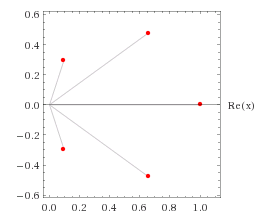
\includegraphics[width=0.5\textwidth]{pentagon}
}\end{center}

\filbreak\begin{enumerate}[resume]
  \answer Show that all solutions to $ (z + 1)^n = z^n $ lie on the line $ \realp{z} = -\frac{1}{2} $.
\end{enumerate}
\begin{align*}
  1 &= \left( \frac{z + 1}{z} \right)^n\\
    &= \left( 1 + \frac{1}{z} \right)^n.
\end{align*}

Now, let $ 1 + \frac{1}{z} = r \cis \theta $. This implies that $ r = 1 $ and $ \theta = \frac{2\pi k}{n} $,
for some integer $ k $:
\begin{align*}
  1 + \frac{1}{z} &= \cis \frac{2\pi k}{n}\\
                  &= \cos \frac{2\pi k}{n} + i\sin \frac{2\pi k}{n}\\
                  &= 1 - 2\sin^2 \frac{\pi k}{n} + 2i \sin \frac{\pi k}{n} \cos \frac{\pi k}{n}\\
      \frac{1}{z} &= 2i\sin \frac{\pi k}{n} \left(\cos \frac{\pi k}{n} + i\sin \frac{\pi k}{n} \right)\\
               z  &= \frac{1}{2i\sin \frac{\pi k}{n} \left(\cos \frac{\pi k}{n} + i\sin \frac{\pi k}{n} \right)}\\
                  &= \frac{1}{2i\sin \frac{\pi k}{n} \cis \frac{\pi k}{n}}\\
                  &= \frac{\cis \frac{-\pi k}{n}}{2i\sin \frac{\pi k}{n} }\\
                  &= \frac{\cos \frac{\pi k}{n} - \sin \frac{-\pi k}{n}}{2i\sin \frac{\pi k}{n} }\\
                  &= \frac{\cos \frac{\pi k}{n}}{2i\sin \frac{\pi k}{n} } - \frac{i\sin \frac{\pi k}{n}}{2i\sin \frac{\pi k}{n} }\\
                  &= \frac{\cos \frac{\pi k}{n}}{2i\sin \frac{\pi k}{n} } - \frac{1}{2}
\end{align*}
so $ \realp{z} = -\frac{1}{2} $, as required.

\filbreak\begin{enumerate}[resume]
  \answer Find all the third roots of 2.
\end{enumerate}

We have that $ \sqrt[3]{2} = 1.259992... $ is one third root of 2. The other
two will be $ \alpha\sqrt[3]{2} = \sqrt[3]{2} \cis \frac{2\pi}{3} $ and
$ \alpha^2\sqrt[3]{2} = \sqrt[3]{2} \cis \frac{4\pi}{3} $.

\filbreak\begin{enumerate}[resume]
  \answer A \textit{group} is a set $ G $ together with some operation $ \cdot $ satisfying the following:
        \begin{enumerate}
          \item For all $ a, b $ in $ G $, $ a \cdot b $ is in $ G $.
          \item For all $ a, b, c $ in $ G $, $ a \cdot (b \cdot c) = (a \cdot b) \cdot c $.
          \item There is some element $ e $ in $ G $ such that for all $ a $ in $ G $, $ a \cdot e = a $.
          \item For every element $ a $ in $ G $ there is some $ b $ in $ G $ such that $ a \cdot b = e $.
        \end{enumerate}
       Show that the set of all $ n$th roots of unity form a group under multiplication.\label{ex:grpdefn}
\end{enumerate}
\paragraph{(a)}
Suppose $ a $ and $ b $ are $n$th roots of unity. Then $ (ab)^n = a^n b^n = 1 $, so $ ab $ is also an $ n$th root of unity.
\paragraph{(b)}
This follows from the associativity of multiplication of complex numbers in general (which in turn follows from associativity
of multiplication of reals).
\paragraph{(c)}
Obviously $ e = 1 $.
\paragraph{(d)}
Suppose $ a $ is an $ n$th root of unity. Then $ a^{-1} $ is also an $ n$th root of unity ($ (a^{-1})^n = (a^n)^{-1} = 1 $),
and $ a a^{-1} = 1 $. Hence $ a^{-1} $ is the required $ b $.

\filbreak\begin{enumerate}[resume]
  \answer Let $ U $ be the set of all complex numbers $ u = a + bi $ such that $ a^2 + b^2 = 1 $.
        \begin{enumerate}
          \answerb Describe all elements of the form $ (3 + 4i)u $ for some $ u $ in $ U $.
          \answerb Describe all elements of the form $ (c + di)u $ for some $ u $ in $ U $.
        \end{enumerate}
\end{enumerate}

\paragraph{(a)}
Note that $ \abs{u} = 1 $ for all $ u $ in $ U $. Hence $ u = \cis \theta $ for some angle,
and $ (3 + 4i)u $ is just $ 5 \cis [\theta + \carg(3 + 4i)] $. But we can pick any $ \theta $,
so the set of all elements of the form $ (3 + 4i)u $ is just all complex numbers of modulus 5.

\paragraph{(b)}
By the same reasoning, the set of all elements of the form $ (c + di)u $ is just all complex numbers of modulus $ \sqrt{c^2 + d^2} $.

\filbreak\begin{enumerate}[resume]
  \answer Suppose $ \sigma(n) $ is the function that sends $ n $ to the sum of its divisors. For example,
        the divisors of 4 are 1, 2, and 4; so $ \sigma(4) = 1 + 2 + 4 = 7 $. Prove that if $ p $ is
        prime then $ \sigma(p^n) = \frac{p^{n+1} - 1}{p - 1} $.
\end{enumerate}
The divisors of $ p^n $ are simply $ 1,~p,~p^2,\dots,~p^n $. Hence $ \sigma(n) = 1 + p + \cdots + p^n = \frac{p^{n + 1} - 1}{p - 1} $.
Note here that we are viewing this sum as a polynomial in a known number $ p $ rather than an indeterminant $ x $.

\section{The Double-Triangle Problem}
There are no exercises for this section that require worked answers.

\section{(Optional) Solving the Cubic}
\begin{enumerate}
  \answer Check the author's algebra.
\end{enumerate}

If the reader is expecting a solution to this problem, she is missing the point.

\filbreak\begin{enumerate}[resume]
  \answer Solve $ t^3 + t^2 - 89t + 231 = 0 $.
\end{enumerate}

We have $ \sigma_1 = -1 $, $ \sigma_2 = -89 $, and $ \sigma_3 = -231 $. Hence,
following the method, we have $ uv = ((-1)^2 - 3(-89))^3 = 19248832 $ and
$ u + v = 2(-1)^3 - 9(-1)(-89) + 27(-231) = -7041 $. Hence, we have
\begin{displaymath}
  u,v = \frac{-7041 \pm \sqrt{(-7041)^2 - 4(19248832)}}{2}
\end{displaymath}
and, plugging these values directly in, we have
\small
\begin{align*}
      x &= \frac{1}{3}\left( -1 + \sqrt[3]{\frac{-7041 + \sqrt{(-7041)^2 - 4(19248832)}}{2}}
                                + \sqrt[3]{\frac{-7041 - \sqrt{(-7041)^2 - 4(19248832)}}{2}} \right)\\
      y &= \frac{1}{3}\left( -1 + \alpha\sqrt[3]{\frac{-7041 + \sqrt{(-7041)^2 - 4(19248832)}}{2}}
                                + \alpha^2\sqrt[3]{\frac{-7041 - \sqrt{(-7041)^2 - 4(19248832)}}{2}} \right)\\
      z &= \frac{1}{3}\left( -1 + \alpha^2\sqrt[3]{\frac{-7041 + \sqrt{(-7041)^2 - 4(19248832)}}{2}}
                                + \alpha\sqrt[3]{\frac{-7041 - \sqrt{(-7041)^2 - 4(19248832)}}{2}} \right)
\end{align*}
\normalsize

So (the author confidently exclaims, after wrestling with his calculator for several minutes) $ x = 7 $, $ y = -11 $,
and $ z = 3 $. It is up to the reader to verify that these are indeed solutions of the original polynomial.

\filbreak\begin{enumerate}[resume]
  \answer Solve $ t^3 + 21t^2 - 32t + 3510 = 0 $.
\end{enumerate}

We have $ \sigma_1 = -21 $, $ \sigma_2 = -32 $, $ \sigma_3 = -3510 $. So $ u + v = -119340 $
and $ uv = 154854153 $. The engineers and physicists among the readers may be tempted to round off, but this
feeling must be controlled.

After plugging everything into the quadratic formula, followed by the cubic formula,
we obtain the three roots $ t \in \{-27, 3+11i, 3-11i\} $.

\filbreak\begin{enumerate}[resume]
  \answer Solve $ 2t^3 + 4it^2 + 58t - 84i $.
\end{enumerate}

We have $ \sigma_1 = -2i $, $ \sigma_2 = 29 $, and $ \sigma_3 = 42i $. Hence
$ u + v = 1672i $ and $ uv = -753571 $.

We calculate the roots as $ t \in \{-7i, 2i, 3i\} $, noting that we need to take
all nine possible combinations of roots, checking to see which three actually
work in the original equation.

\filbreak\begin{enumerate}[resume]
  \answer In 1225, Leonardo of Pisa (Fibonacci) was asked by Holy Roman Emperor Frederick II
        to solve the cubic equation $ x^3 + 2x^2 + 10x = 20 $. His solution was
        \begin{displaymath}
          x = 1 + \frac{22}{60} + \frac{7}{60^2} + \frac{42}{60^3} + \frac{33}{60^4} + \frac{4}{60^5} + \frac{40}{60^6}.
        \end{displaymath}
        \begin{enumerate}
          \answerb Show that the equation has exactly one real root.
          \answerb Use the method outlined in this section to find numerical approximations to the three roots
                of the polynomial.
        \end{enumerate}
\end{enumerate}

\paragraph{(a)}
We wish to show that the graph of $ y = x^3 + 2x^2 + 10x - 20 $ crosses the $ x$-axis exactly
one time. We find that $ \od{y}{x} = 3x^2 + 4x + 10 $ has no real roots, and so the graph of
$ y $ has no turning points. Since $ y $ is continuous, it must be strictly increasing and
therefore crosses the $ x$-axis exactly once.

\paragraph{(b)}
This question is nasty.

$ \sigma_1 = -2 $, $ \sigma_2 = 10 $, $ \sigma_3 = 20 $.

\begin{align*}
  u + v &= 704\\
  uv &= -17576\\
  \\
  u &\approx 728.1383\\
  v &\approx -24.13827
\end{align*}

Possible roots:

\begin{tabular}{r|c c c|}
  & $ 1 $ & $ \omega $ & $ \omega^2 $\\
  \hline
  $ 1 $ & \cellcolor{Emerald!25} $ 1.368808 $ & $ 2.813822 - 0.8342792i $ & $ 2.813822 + 0.8342792i $\\
  $ \omega $ & $ -3.129418 + 2.597052i $ & $ -1.68404 + 1.762773i $ & \cellcolor{Emerald!25} $ -1.68404 + 3.431332i $\\
  $ \omega^2 $ & $ -3.129418 - 2.597052i $ & \cellcolor{Emerald!25} $ -1.68404 - 3.431332i $ & $ -1.68404 + -.762773i $
\end{tabular}

\filbreak\begin{enumerate}[resume]
  \answer Solve $ t^3 - 15t - 4 = 0 $ using the methods outlined in this section. See exercise \ref{ex:cardano}
        from the section on complex numbers.
\end{enumerate}

$ \sigma_1 = -2 $, $ \sigma_2 = 10 $, $ \sigma_3 = 20 $.

\begin{align*}
  u + v &= 108\\
  uv &= 91125
\end{align*}

The working roots are $ t \in \{ 4, -2 + \sqrt{3}, -2 - \sqrt{3} \} $.

\filbreak\begin{enumerate}[resume]
  \answer Verify that $ uv $ and $ u + v $ are symmetric in $ x $, $ y $, and $ z $.
\end{enumerate}
This can be done by expanding both expressions out in terms of $ x $, $ y $, and $ z $ (the expressions
themselves are given in the text, $ \sigma_k $ terms can be substituted out) and checking that
for each type of term, all possible combinations of the three variables occur. For example, if $ xy $
occurs then $ xz $ and $ yz $ must also appear.

\filbreak\begin{enumerate}[resume]
  \answer Read the historical introduction of Ian Stewart's \textit{Galois Theory}.
\end{enumerate}
For bonus marks, read the book and list all the typoes\footnote{~An intentional mispelling.}.

\filbreak\begin{enumerate}[resume]
  \answer The discriminant of the general quartic equation $ q(x) = A(x - \alpha)(x - \beta)(x - \gamma)(x - \delta) $ is
        given by the formula
        \begin{displaymath}
          \Delta_4 [q(x)] = (\alpha - \beta)^2(\alpha - \gamma)^2(\alpha - \delta)^2(\beta - \gamma)^2(\beta - \delta)^2(\gamma - \delta)^2.
        \end{displaymath}
        Suppose that for a particular quartic $ Q(x) $ with real coefficients, $ \Delta_4[Q(x)] > 0 $. What can you say about the number of real roots?
\end{enumerate}
Firstly, there must be no repeated roots (or the discriminant would be zero).

Obviously if all four roots are real, the discriminant is positive (since it is a square); so suppose that there is at least one complex root.
We know that any non-real roots must appear in conjugate pairs. Let the four roots be $ a \pm bi $ and $ c \pm di $, so (after simplifying)
\begin{align*}
  \Delta_4 [q(x)] &= (a + bi - a + bi)^2  (a + bi - c - di)^2  (a + bi - c + di)^2\\&\qquad  (a - bi - c - di)^2  (a - bi - c + di)^2  (c + di - c + di)^2\\
                  &= 16b^2d^2(a^4 - 4a^3c + 2a^2b^2 + 6a^2c^2 + 2a^2d^2 - 4ab^2c - 4ac^3\\&\qquad - 4acd^2 + b^4 + 2b^2c^2 - 2b^2d^2 + c^4 + 2c^2d^2 + d^4)^2
\end{align*}
But $ \Delta_4 [q(x)] \neq 0 $, so neither $ b $ nor $ d $ is zero. Hence all four roots are complex.

Therefore if the discriminant is positive, either all four roots are real or all four roots are complex.

\section{Final Exercises}
\begin{enumerate}
  \answer Is $ (x-15) $ a factor of $ (x^3 - 19x - 30) $? Is $ (x^2 + 5x + 6) $ a factor?
\end{enumerate}

By the remainder theorem, $ (x-15) $ is not a factor ($15^3 - 19(15) - 30 = 3060 \neq 0 $).
We check each factor of $ (x^2 + 5x + 6) $ individually:
\begin{align*}
  (-2)^3 - 19(-2) - 30 &= 0\\
  (-3)^3 - 19(-3) - 30 &= 0
\end{align*}
So the quadratic is a factor.

\filbreak\begin{enumerate}[resume]
  \answer Factor completely $ 9x^4 - 13x^2 + 4 $.
\end{enumerate}

Using the quadratic formula, $ x^2 \in \{\frac{4}{9}, 1\} $ and so
$ x \in \{-1, -\frac{2}{3}, \frac{2}{3}, 1\} $. Hence the full factorisation
is $ (x+1)(x-1)(x+\frac{2}{3})(x-\frac{2}{3}) $.

\filbreak\begin{enumerate}[resume]
  \answer Solve $ x^3 + 9x^2 = 60 - 8x $.
\end{enumerate}

After trying a few simple solutions, we find that $ x = 2 $ is a solution.

\polylongdiv{x^3 + 9x^2 + 8x - 60}{x - 2}

We factor the quadratic as $ (x+5)(x+6) $, so the three solutions of the
cubic are $ x \in\{-6,-5,2\} $.

\filbreak\begin{enumerate}[resume]
  \answer Find $ k $ such that $ (x - 4) $ is a factor of $ x^3 + 7x^2 - 14x + k $.
\end{enumerate}

By the remainder theorem, we want $ 4^3 + 7(4)^2 - 14(4) + k = 0 $. Hence $ k = -120 $.

\filbreak\begin{enumerate}[resume]
  \answer Find a value of $ k \neq 0 $ such that $ kx^2 -6x + 1 = 0 $ will have just one root.
\end{enumerate}

We set $ \Delta_2 = (-6)^2 - 4k = 0 $, so $ k = 9 $.

\filbreak\begin{enumerate}[resume]
  \answer Find all sixth roots of $ i $.
\end{enumerate}

We convert to polar form, so $ i = \cis \frac{\pi}{2} $. Then, by de Moivre's
Theorem, we have:

\begin{center}
\begin{tabular} {c | c}
  \textbf{Root} & \textbf{Polar form}\\
  $ z_1 $ & $ \cis \frac{\pi}{12} $    \\
  $ z_2 $ & $ \cis \frac{5\pi}{12} $   \\
  $ z_3 $ & $ \cis \frac{3\pi}{4} $    \\
  $ z_4 $ & $ \cis \frac{13\pi}{12} $  \\
  $ z_5 $ & $ \cis \frac{17\pi}{12} $  \\
  $ z_6 $ & $ \cis \frac{7\pi}{4} $
\end{tabular}
\end{center}

\filbreak\begin{enumerate}[resume]
  \answer Find $ k $ such that $ 8 - x +  2\sqrt{2x + k} = 0 $ has exactly one real root.
\end{enumerate}
Rearrange as follows:
\begin{align*}
  2\sqrt{2x + k} &= x - 8\\
  8x + 4k &= x^2 - 16x + 64\\
  0 &= x^2 - 24x + (64 - 4k)
\end{align*}
But $ \Delta_2 = 0 $, so $ 24^2 = 4(64 - 4k) $ and $ k = -20 $.

\filbreak\begin{enumerate}[resume]
  \answer Solve $ (\alpha^2 + 2\alpha -4)(\alpha^7 + 1) = 0 $.
\end{enumerate}

The roots of the first factor are $ \alpha = -1 \pm \sqrt{5} $. The roots
of the second are simply all the seventh roots of unity, so all nine roots of
the equation are:
\begin{center}
\begin{tabular} {c | c | c}
  \textbf{Root} & \textbf{Polar form} & \textbf{Rectangular form}\\
  $ z_8 $ && $ -1 + \sqrt{5} $        \\
  $ z_9 $ && $ -1 - \sqrt{5} $        \\
  $ z_1 $ &  $ \cis 0 $ & 1           \\
  $ z_2 $ &  $ \cis \frac{2\pi}{7} $  \\
  $ z_3 $ &  $ \cis \frac{-2\pi}{7} $ \\
  $ z_4 $ &  $ \cis \frac{4\pi}{7} $  \\
  $ z_5 $ &  $ \cis \frac{-4\pi}{7} $ \\
  $ z_6 $ &  $ \cis \frac{6\pi}{7} $  \\
  $ z_7 $ &  $ \cis \frac{-6\pi}{7} $
\end{tabular}
\end{center}

\filbreak\begin{enumerate}[resume]
  \answer Solve $ x^4 + x^2 + 1 = 0 $ for $ x $.
\end{enumerate}

$ x^2 = \frac{-1\pm\sqrt{3}i}{2} $, so $ x = \pm\frac{1\pm\sqrt{3}i}{2} $.

\filbreak\begin{enumerate}[resume]
  \answer Solve $ \beta^2 + \beta + 1 = 0 $ for $ x $ if $ \beta = x^2 + x + 1 $.
\end{enumerate}

We have $ \beta = \frac{-1}{2}\pm\frac{\sqrt{3}i}{2} $.
Now, $ x^2 + x + 1.5 \mp \frac{\sqrt{3}{i}}{2} = 0 $.

Using the quadratic formula (twice!), we obtain the following four roots:
\begin{center}
\begin{tabular} {c | c}
  \textbf{Root} & \textbf{Rectangular form}\\
  $ x_1 $ & $ \frac{-1+\sqrt{-5-2\sqrt{3}i}}{2} $    \\
  $ x_2 $ & $ \frac{-1-\sqrt{-5-2\sqrt{3}i}}{2} $   \\
  $ x_3 $ & $ \frac{-1+\sqrt{-5+2\sqrt{3}i}}{2} $    \\
  $ x_4 $ & $ \frac{-1-\sqrt{-5+2\sqrt{3}i}}{2} $
\end{tabular}
\end{center}

\filbreak\begin{enumerate}[resume]
  \answer Let $ \alpha $, $ \beta $, and $ \gamma $ be the three roots of $ ax^3 + bx^2 + cx + d = 0 $. Prove that:
        \begin{enumerate*}
          \answerb $ \alpha + \beta + \gamma = \frac{-b}{a} $,
          \answerb $ \alpha\beta + \beta\gamma + \alpha\gamma = \frac{c}{a} $, and
          \answerb $ \alpha\beta\gamma = \frac{-d}{a} $.
        \end{enumerate*}
        Hence show that $ \alpha^2\beta\gamma + \alpha\beta^2\gamma + \alpha\beta\gamma^2 = \frac{bd}{a^2} $.
\end{enumerate}

We have that $ ax^3 + bx^2 + cx + d = a(x - \alpha)(x - \beta)(x - \gamma) = ax^3 - a(\alpha + \beta + \gamma)x^2 + a(\alpha\beta + \alpha\gamma + \beta\gamma)x - a\alpha\beta\gamma $,
and so $ b = - a(\alpha + \beta + \gamma) $, $ c = a(\alpha\beta + \alpha\gamma + \beta\gamma) $, and $ d = - a\alpha\beta\gamma $.

Hence, $ \frac{-b}{a} = \frac{a(\alpha + \beta + \gamma)}{a} = \alpha + \beta + \gamma $,
       $ \frac{c}{a} = \frac{a(\alpha\beta + \alpha\gamma + \beta\gamma)}{a} = \alpha\beta + \alpha\gamma + \beta\gamma $, and
       $ \frac{-d}{a} = \frac{a\alpha\beta\gamma}{a} = \alpha\beta\gamma $ as expected.

We also have that $ \frac{bd}{a^2} = \frac{-b}{a} \times \frac{-d}{a} = (\alpha + \beta + \gamma)\alpha\beta\gamma = \alpha^2\beta\gamma + \alpha\beta^2\gamma + \alpha\beta\gamma^2 $.

\filbreak\begin{enumerate}[resume]
  \answer Solve $ (z+1)^3 = 8(z-1)^3 $ for $ z $. Give exact answers in the form $ a + ib $.
\end{enumerate}

Expanding, $ z^3 + 3z^2 + 3z + 1 = 8z^3 - 24z^2 + 24z - 8 $ and so we need to solve
$ 7z^3 -27z^2 + 21z - 9 = 0 $. Using magic, we notice that one solution is $ z = 3 $ ---
a useful trick is to realise that there must be at least one real root (as we have an odd
polynomial with real coefficients), and that that root must divide the constant term: this
means we only need to try $ z = 1 $, $ z = 3 $, and $ z = 9 $ (and the negatives of those values).

Dividing:
\polylongdiv[vars=z]{7z^3 -27z^2 + 21z - 9}{z-3}

Using the quadratic formula, we find the roots of the quadratic factor to be
$ z = \frac{3}{7} \pm \frac{2}{7}\sqrt{3}i $.

\filbreak\begin{enumerate}[resume]
  \answer Graph the equation $ \abs{z} = 3 $ in the complex plane.
\end{enumerate}

\begin{center}\fbox{
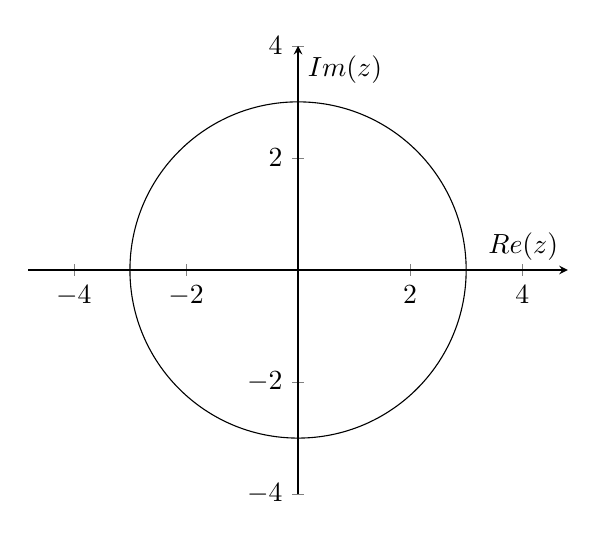
\begin{tikzpicture}
  \begin{axis}[
    xlabel=$Re(z)$,
    ylabel={$Im(z)$},
    axis lines=middle,
    disabledatascaling,
    xmin=-4,
    xmax=4,
    ymin=-4,
    ymax=4,
    axis equal
  ]
  \path [draw=black, fill=none] (0,0) circle (3);
  \end{axis}
\end{tikzpicture}
}\end{center}

\filbreak\begin{enumerate}[resume]
  \answer If $ z = 1+i $ and $ w = \frac{1}{z} + i $, find the argument of $ w $.
\end{enumerate}
\begin{align*}
  w &= \frac{1}{1+i} + i\\
    &= \frac{1-i}{(1+i)(1-i)} + i\\
    &= \frac{1-i}{2} + i\\
    &= \frac{1}{2} + \frac{1}{2}i\\
  \Rightarrow \carg{w} &= \frac{\pi}{4}.
\end{align*}

\filbreak\begin{enumerate}[resume]
  \answer If $ \frac{z + 2i}{z-2i} $ is purely imaginary, describe the possible values of $ z $.
\end{enumerate}

Let $ z = x + yi$.

\begin{align*}
  \frac{x+(y+2)i}{x+(y-2)i} &= \frac{(x+(y+2)i)(x-(y-2)i)}{(x+(y-2)i)(x-(y-2)i)}\\
                            &= \frac{x^2 + x(y+2)i - x(y-2)i + (y+2)(y-2))}{x^2+(y-2)^2}\\
                            &= \frac{x^2 + 4ix + y^2 - 4}{x^2+(y-2)^2}
\end{align*}

So in order for the fraction to be purely imaginary, $ x^2 + y^2 = 4 $ and so $ z $ must
lie on the circle of radius two centred on the origin.

\filbreak\begin{enumerate}[resume]
  \answer If $ \abs{z - 1 + 2i} = \abs{z + 1} $ and $ z = x+yi $, find an expression for $ y $ in terms
        of $ x $ (i.e. find the locus of $ z $).
\end{enumerate}
\begin{align*}
  \abs{(x-1) + (y+2)i} &= \abs{(x+1) + yi} \\
  \sqrt{(x-1)^2 + (y+2)^2} &= \sqrt{(x+1)^2 + y^2}\\
  x^2 - 2x+ 1 + y^2 + 4y + 4 &= x^2 + 2x + 1 + y^2\\
  4y &= 4x- 4\\
  y &= x - 1.
\end{align*}

\filbreak\begin{enumerate}[resume]
  \answer Sketch the region satisfied by $ \realp{z - i \bar z} > 2 $.
\end{enumerate}
Let $ z = x + yi $.
\begin{align*}
  z - i \bar z &= x + yi - xi + y\\
  \realp{z - i \bar z} &= x + y
\end{align*}

So the region is $ x + y > 2 $:

\begin{center}
  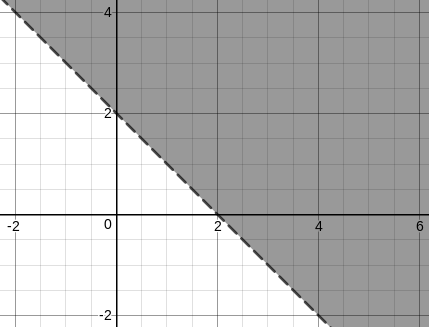
\includegraphics[width=0.5\textwidth]{inequality}
\end{center}


\filbreak\begin{enumerate}[resume]
  \answer If $ x = 2 $ and $ x = 6 $ are solutions of $ p(x) = Ax^2 + Bx + C $ and $ p(0) = -4 $,
        find $ A $, $ B $, and $ C $.
\end{enumerate}

A quadratic equation with the roots $ x = 2 $ and $ x = 6 $ must have the form
$ A(x-2)(x-6) = Ax^2 - 8Ax + 12A $, and the constant term $ p(0) = C = 12A = -4 $.

Hence $ A = \frac{-4}{12} = -\frac{1}{3} $, and so $ p(x) = \frac{-x^2}{3} + \frac{8x}{3} - 4 $.


\filbreak\begin{enumerate}[resume]
  \answer If $ w = 2-3i $ is a zero of $ 3w^3 - 14w^2 + Aw - 26 $ (where $ A $ is real), find $ A $
        and the remaining two roots.
\end{enumerate}

Given that the polynomial has real coefficients, $ \bar w = 2+3i $ must also be a root. Call $ \alpha $
the third (and only real) root.

We can expand the factored form and equate the coefficients:
\begin{align*}
  (x - 2+3i)(x - 2-3i)(x - \alpha) &= (x^2 -4x + 13)(x - \alpha)\\
                                   &= x^3 - x^2(4+\alpha) + x(14 + 4\alpha) - 13\alpha
\end{align*}
So $ \alpha = 2 $ and $ A = 13 + 4\times2 = 21 $.

\filbreak\begin{enumerate}[resume]
  \answer Use de Moivre's Theorem to show that
        \begin{enumerate}
          \answerb $ \sin 2\theta = 2\sin\theta\cos\theta $ and $ \cos 2\theta = \cos^2 \theta - \sin^2 \theta $; and
          \answerb $ \sin 3\theta = 3\sin\theta - 4\sin^3\theta $ and $ \cos 3\theta = 4\cos^3\theta - 3\cos\theta $.
        \end{enumerate}
\end{enumerate}

\paragraph{(a)}
The key idea is to note that we can expand $ \cis^n \theta $ in two different ways: by the binomial
theorem, and by de Moivre's theorem.
\begin{align*}
  \cis 2\theta &= (\cis \theta)^2\\
               &= (\cos \theta + i\sin \theta)^2\\
               &= \cos^2 \theta + 2i\cos\theta\sin\theta - \sin^2 \theta
\end{align*}
Taking just the real parts, we obtain $ \cos 2\theta = \cos^2 \theta - \sin^2 \theta $, and
taking just the non-real parts, we obtain $ \sin 2\theta = 2\cos\theta\sin\theta $ as expected.

\paragraph{(b)}
Likewise for the third power (although we use identities to simplify further):
\begin{align*}
  \cis 3\theta &= (\cis \theta)^3\\
               &= (\cos \theta + i\sin \theta)^3\\
               &= \cos^3 \theta + 3i   \cos^2\theta \sin\theta - 3\cos\theta    \sin^2\theta  - i\sin^3\theta\\
               &= \cos^3 \theta + 3i(1-\sin^2\theta)\sin\theta - 3\cos\theta (1-\cos^2\theta) - i\sin^3\theta\\
               &= 4\cos^3 \theta + 3i \sin\theta - 3\cos\theta - 4i \sin^3 \theta
\end{align*}
Hence $ \cos 3\theta = 4\cos^3 \theta - 3\cos\theta $ and $ \sin 3\theta = 3\sin\theta - 4\sin^3\theta $.

\filbreak\begin{enumerate}[resume]
  \answer Use Euler's formula to prove that $ \cos(\alpha + \beta) = \cos \alpha \cos \beta - \sin \alpha \sin \beta $, and that
        $ \sin(\alpha + \beta) = \sin \alpha \cos \beta + \cos \alpha \sin \beta $.
\end{enumerate}

\begin{align*}
  \cos (\alpha + \beta) + i\sin (\alpha + \beta) = e^{i(\alpha + \beta)} &= e^{i\alpha}  e^{i\beta}\\
                                                &= (\cos \alpha + i \sin \alpha)(\cos \beta + i \sin \beta)\\
                                                &= \cos \alpha \cos \beta + i \sin \alpha \cos \beta + i \cos\alpha \sin \beta - \sin \alpha \sin \beta\\
                                                &= (\cos \alpha \cos \beta - \sin \alpha \sin \beta) + i(\sin\alpha\cos\beta + \sin\beta\cos\alpha).
\end{align*}
The identities immediately follow from equating real and imaginary components.

\filbreak\begin{enumerate}[resume]
  \answer Show that $ \arctan a + \arctan b = \arctan \frac{a + b}{1 - ab} $.
\end{enumerate}

Recall that $ \carg (x + yi) = \arctan \frac{y}{x} $. Specifically, $ \carg(1 + yi) = \arctan y $.
Hence, we argue as follows:
\begin{align*}
  \arctan a + \arctan b &= \carg(1 + ai) + \carg(1 + bi) \\
                        &= \carg((1 + ai)(1 + bi))\\
                        &= \carg((1 - ab) + (a + b)i)\\
                        &= \arctan \frac{a + b}{a - ab}.
\end{align*}

\textbf{Aside: }
Note that $ \carg $ here behaves like a logarithm in that it converts a sum to a product. This
is because if $ z = \cis \theta $ then $ z = e^{i\theta} $ and so $ \carg z = \theta = \frac{1}{i} \ln z $;
hence we take $ \carg w + \carg z = \frac{1}{i}{\ln w + \ln z} = \frac{1}{i} \ln (wz) = \carg wz $.

\filbreak\begin{enumerate}[resume]
  \answer Suppose that $ \abs{z+w} = \abs{z-w} $. Show that $ \carg z - \carg w = \pm \frac{\pi}{2} $.
\end{enumerate}

\paragraph{Proof using the $ \arctan $ result from the previous exercise.}
Let $ z = a+bi $ and $ w = c+di $.
\begin{align*}
  \carg z - \carg w &= \arctan \left( \frac{b}{a} \right) - \arctan \left( \frac{d}{c} \right)\\
                    &= \arctan \left( \frac{\frac{b}{a} - \frac{d}{c}}{1+ \frac{bd}{ac}} \right).
\end{align*}
We therefore have that $ \pm \frac{\pi}{2} = \arctan \left( \frac{\frac{b}{a} - \frac{d}{c}}{1+ \frac{bd}{ac}} \right) $,
and therefore $ \tan \left( \pm \frac{\pi}{2} \right) = \frac{\frac{b}{a} - \frac{d}{c}}{1+ \frac{bd}{ac}} $. However, note that
$ \tan \left( \pm \frac{\pi}{2} \right) $ is undefined; a sufficient reason for this would be the denominator of the fraction on the
right hand side becoming zero, which occurs when $ \frac{bd}{ac} = -1 $. Hence, if we can show this last fact, we
imply that $ \carg z - \carg w = \pm \frac{\pi}{2} $.

This can be done as follows:
\begin{align*}
  \abs{z + w} = \abs{z - w} &\Rightarrow \abs{a + bi + c + di} = \abs{a + bi - c - di}\\
                            &\Rightarrow \sqrt{(a+c)^2 + (b+d)^2} = \sqrt{(a-c)^2 + (b-d)^2}\\
                            &\Rightarrow a^2 + 2ac + c^2 + b^2 + 2bd + d^2 = a^2 - 2ac + c^2 + b^2 - 2bd + d^2\\
                            &\Rightarrow 4ac = -4bd\\
                            &\Rightarrow \frac{bd}{ac} = -1.
\end{align*}

\paragraph{Geometric proof.}
Consider the addition parallelogram formed by $ u $ and $ v $.
\begin{center}
  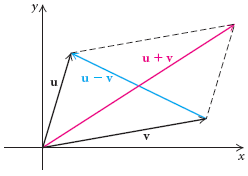
\includegraphics[width=0.5\textwidth]{vecadd}\\
\end{center}
The lengths of the two diagonals of a parallelogram can only be equal
if the parallelogram is in fact a square; i.e. $ u $ and $ v $ are at
right angles, and so the angle between them will be $ \frac{\pi}{2} $.


\filbreak\begin{enumerate}[resume]
  \answer  If $ 3z^3 + (2-3ai)z^2 + (6+2bi)z + 4 $ has exactly one real root, what value must
        the quotient $ b/a $ take if both $ a $ and $ b $ are real? Find the real root.
\end{enumerate}

For a real root to occur, the imaginary part of the polynomial must become zero (assuming $ z \in \mathbb{R} $).
Hence we first solve $ -3aiz^2 + 2biz = 0 $, finding the two solutions to be $ z = 0 $ and $ z = \frac{2b}{3a} $.

Looking at the real part, we need to solve $ 3z^3 + 2z^2 + 6z + 4 = 0 $; $ z = 0 $ is not a solution here, so that
means that in order to find the single remaining possible real root we must find $ \frac{2b}{3a} $. Luckily this cubic
does not have coefficients depending on $ a $ or $ b $ (so we can find exact answers), and so we solve it to find that
it has a single real solution of $ z = -\frac{2}{3}$; so the single real root is $ z = -\frac{2}{3} $ and $ \frac{b}{a} = -1 $.

\filbreak\begin{enumerate}[resume]
  \answer Complex numbers exist in a plane, and so can be used to solve problems in geometry. For example, multiplication
        by $ i $ rotates a point by $ \frac{\pi}{2} $ around the origin. A generalisation of this allows us to rotate
        a point $ z $ around an arbitrary point $ a $ by that angle: $ z' = a + i(z-a) $.

        A pirate named Kim Dotcom has hidden his sick tunes on a desert island tax haven in order to evade
        American FBI agents. You have been hired to find the data stick containing his mp3 files so that
        his extradition case can be resolved, but all you can find is a treasure map with the following
        instructions:

        \begin{aquote}{Kim Dotcom's Amazing Totally Secret Treasure Map\textsuperscript{TM}}
          From the statue of Richard Seddon, go to the kauri tree (counting your steps), and then turn
          exactly 90\degree left and walk the same number of steps to the point $ g' $. Returning
          to the statue, walk to the beech tree (again counting your steps). Turn right by 90\degree,
          and walk the same number of steps to point $ g'' $. The treasure is buried exactly at the midpoint
          of the line joining $ g' $ and $ g'' $.
        \end{aquote}

        Given that the kauri tree is at $ (0,0) $, the beech tree is at $ (10,0) $, and
        the statue is somewhere on the line $ y = 2009 $, find the location of the treasure
        using the geometry of complex numbers and rid New Zealand of Kim Dotcom forever.\footnote{~Problem taken
        from Kessler (2009) section 5.1, but context changed.}
\end{enumerate}

We will call the $ x$-coordinate of the statue $ x_0 $.

Our technique for solving this problem is simply to rotate the point representing
the statue around the given points for the trees by 90\degree using the formula given
in the question --- then finding the midpoint is simple.

First, we rotate $ x_0 + 2009i $ around the point $ 0 + 0i $, obtaining $ g' = -2009 + ix_0 $.
We next rotate the statue around $ 10 + 0i $ three times (as we are turning
right --- draw a diagram!) using the formula:
\begin{align*}
  10 + i(x_0 + 2009i - 10)         &= -1999 + i(x_0 - 10)\\
  10 + i(-1999 + i(x_0 - 10) - 10) &= 20 - x_0 - 2009i\\
  10 + i(20 - x_0 - 2009i - 10)    &= 2019 + i(10 - x_0)
\end{align*}
The midpoint is therefore $ \left( \frac{-2009 + 2019}{2}, \frac{x_0 + 10 - x_0}{2} \right) = (5,5)$. Interestingly,
the position of the treasure does not depend on the $ x$-coordinate of the statue!

\filbreak\begin{enumerate}[resume]
  \answer A line in $ \mathbb{C}^2 $ (the plane with complex coordinates) is defined to be the locus of a linear
        $ ax + by + c = 0 $ where $ a $, $ b $, and $ c $ are complex constant. Prove that, given two distinct points $ (x_0, y_0) $
        and $ (x_1, y_1) $ in $ \mathbb{C}^2 $, there is a \textbf{unique} line through those two points. \textit{Hint: it is certainly \textbf{not} true
        that there is a unique linear equation whose graph includes both points.}
\end{enumerate}

Let $ \mathcal{L} $ and $ \mathcal{M} $ be two lines passing through both points. (Our goal is to show
that $ (x,y) \in \mathcal{L} \iff (x,y) \in \mathcal{M} $.) Then $ \mathcal{L} $ is the locus of some
linear equation $ ax + by + c = 0 $, and $ \mathcal{M} $ is the locus of some other linear
equation $ dx + ey + f = 0 $.

Consider first $ \mathcal{L} $. We know that $ (x_0, y_0) \in \mathcal{L} \wedge (x_1, y_1) \in \mathcal{L} $. Hence we
have the following system of simultaneous equations:
\begin{align*}
  ax_0 + by_0 + c = 0\\
  ax_1 + by_1 + c = 0.
\end{align*}

Since we have a system of rank two with three variables, one variable must be free (a parameter); we chose it to be $ c $ as this
simplifies the whole process. Our goal, therefore, is to rewrite $ ax + by + c = 0 $ in terms of $ c $ only (the purpose of this
goal may not be clear at this point, but trust us). This can be done using any appropriate method (e.g. substitution); we chose to
use linear algebra because it minimises the amount of tedious work required.

\begin{mdframed}[hidealllines=true,backgroundcolor=Dandelion!20]
\textit{Readers who do not know linear algebra should feel free to skip this portion of the solution, and are encouraged to find
another way to derive the same result.}

We have
\begin{displaymath}
  \begin{bmatrix} x_0 & y_0 \\ x_1 & y_1 \end{bmatrix} \begin{bmatrix} a\\b \end{bmatrix} = \begin{bmatrix} -c\\-c \end{bmatrix}.
\end{displaymath}

Inverting the coefficient matrix and solving for $ (a\ b)^t $ gives
\begin{displaymath}
  \begin{bmatrix} a\\b \end{bmatrix} = \frac{1}{x_0 y_1 - x_1 y_0} \begin{bmatrix} y_1 & -y_0 \\ -x_1 & x_0 \end{bmatrix} \begin{bmatrix} -c\\-c \end{bmatrix};
\end{displaymath}
\end{mdframed}

We therefore conclude that
\begin{align*}
  a &= -\frac{c}{x_0 y_1 - x_1 y_0} (y_1 - y_0)\\
  b &= -\frac{c}{x_0 y_1 - x_1 y_0} (x_0 - x_1)
\end{align*}
and (substituting) $ \mathcal{L} $ is the locus of
\begin{displaymath}
  c \left(1 - \frac{y_1 - y_0}{x_0 y_1 - x_1 y_0} x - \frac{x_0 - x_1}{x_0 y_1 - x_1 y_0} y \right) = 0.
\end{displaymath}
Similarly, $ \mathcal{M} $ is the locus of
\begin{displaymath}
  f \left(1 - \frac{y_1 - y_0}{x_0 y_1 - x_1 y_0} x - \frac{x_0 - x_1}{x_0 y_1 - x_1 y_0} y \right) = 0.
\end{displaymath}

Now, we must show that if a point $ (x_\star, y_\star) $ is in $ \mathcal{L} $ then it is in $ \mathcal{M} $ (and vice versa).
To this end, consider the following:
\begin{displaymath}
  (x_\star, y_\star) \in \mathcal{L} \iff c \left(1 - \frac{y_1 - y_0}{x_0 y_1 - x_1 y_0} x_\star - \frac{x_0 - x_1}{x_0 y_1 - x_1 y_0} y_\star \right) = 0
\end{displaymath}
So one of $ c = 0 $ and $ \left(1 - \frac{y_1 - y_0}{x_0 y_1 - x_1 y_0} x_\star - \frac{x_0 - x_1}{x_0 y_1 - x_1 y_0} y_\star \right) = 0 $ is true.

\paragraph{Case I: $ \left(1 - \frac{y_1 - y_0}{x_0 y_1 - x_1 y_0} x_\star - \frac{x_0 - x_1}{x_0 y_1 - x_1 y_0} y_\star \right) = 0 $}\mbox{}\\
Evidently
\begin{displaymath}
  f \left(1 - \frac{y_1 - y_0}{x_0 y_1 - x_1 y_0} x_\star - \frac{x_0 - x_1}{x_0 y_1 - x_1 y_0} y_\star \right) = 0
\end{displaymath}
and so $ (x_\star, y_\star) \in \mathcal{M} $. (The same argument works with $ \mathcal{M} $ and $ \mathcal{L} $ swapped.)

\paragraph{Case II: $ c = 0 $ and $ \left(1 - \frac{y_1 - y_0}{x_0 y_1 - x_1 y_0} x_\star - \frac{x_0 - x_1}{x_0 y_1 - x_1 y_0} y_\star \right) \neq 0 $}\mbox{}\\
In both cases,
\begin{displaymath}
  f \left(1 - \frac{y_1 - y_0}{x_0 y_1 - x_1 y_0} x_\star - \frac{x_0 - x_1}{x_0 y_1 - x_1 y_0} y_\star \right) = 0
\end{displaymath}
and so $ (x_\star, y_\star) \in \mathcal{M} $. The above arguments also show that $ (x_\star, y_\star) \in \mathcal{M} \implies (x_\star, y_\star) \in \mathcal{L} $,
so $ \mathcal{M} = \mathcal{L} $.

\filbreak\begin{enumerate}[resume]
  \answer Find all possible values for $ \theta $ if $ \cis^2 \theta + \cis \theta + 1 = 0 $.
\end{enumerate}

We have a quadratic in $ \cis \theta $, so $ \cis \theta = \frac{-1\pm\sqrt{3}i}{2} $.

Hence $ \cos \theta = \frac{-1}{2} $ and $ \sin \theta = \frac{\sqrt{3}}{2} $,
so $ \theta = \frac{2\pi}{3} + 2n\pi $ for $ n \in \mathbb{N} $.

\filbreak\begin{enumerate}[resume]
  \answer Graph the locus of $ \carg w = \abs{w} $. What about $ \carg w + \abs{w} = 1 $?
\end{enumerate}

The first equation (in black) is an equiangular spiral; the second (in green) is congruent to the first spiral but transformed.

\begin{center}\fbox{
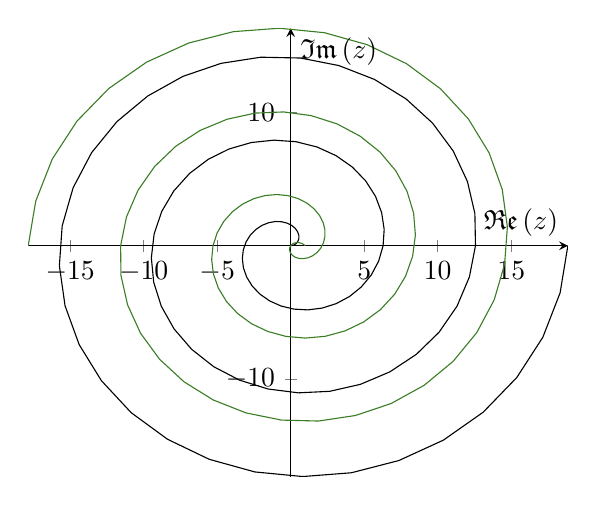
\begin{tikzpicture}
  \begin{axis}[
     xlabel=$\realp{z}$,
     ylabel={$\imagp{z}$},
     xlabel near ticks,
     ylabel near ticks,
     axis lines=middle,
  ]
    \addplot[domain=0:6*pi, samples=100, color=black, data cs=polarrad]{x};
    \addplot[domain=0:6*pi, samples=100, color=OliveGreen, data cs=polarrad]{1-x};
  \end{axis}
\end{tikzpicture}
}\end{center}

\filbreak\begin{enumerate}[resume]
  \answer Given a quadratic equation $ x^2 + px + q $ and a root $ \alpha $, show that the other root $ \beta $ is
        given by $ \beta = -p - \alpha $ and find a similar expression for finding two roots of a cubic given the
        third.
\end{enumerate}
The first fact is easily shown by writing out the quadratic in factored form and matching coefficients:
\begin{displaymath}
  (x - \alpha)(x - \beta) = x^2 - (\alpha + \beta)x + \alpha\beta
\end{displaymath}
So $ p = -\alpha -\beta \Rightarrow \beta = -p-\alpha $.
Note we have two equations ($ p = -\alpha - \beta $ and $ q = \alpha\beta $) in \textit{one} unknown (namely $ \beta $),
so the system is easily solvable.

Attempting the same thing for the cubic $ x^3 + px^2 + qx + r $, with the known root being $ \gamma $:
\begin{displaymath}
  (x - \alpha)(x - \beta)(x - \gamma) = x^3 - (\alpha + \beta + \gamma)x^2 + (\alpha\beta + \alpha\gamma + \beta\gamma)x - \alpha\beta\gamma
\end{displaymath}
So we have three equations in two unknowns:
\begin{align*}
  p &= -\alpha - \beta - \gamma\\
  q &= \alpha\beta + \alpha\gamma + \beta\gamma\\
  r &= - \alpha\beta\gamma
\end{align*}
We rearrange and solve the first and third equations to find an expression for $ \alpha $ in terms of
$ \gamma $:
\begin{align*}
  \beta = -p - \alpha - \gamma &= \frac{-r}{\alpha\gamma}\\
  p + \alpha + \gamma &= \frac{r}{\alpha\gamma}\\
  p\alpha\gamma + \alpha^2\gamma + \alpha\gamma^2 - r &= 0\\
  \gamma \alpha^2 + (p\gamma + \gamma^2)\alpha - r &= 0
\end{align*}
Using the quadratic formula:
\begin{align*}
  \alpha = \frac{-p\gamma-\gamma^2 \pm \sqrt{(p\gamma + \gamma^2)^2 + 4r\gamma}}{2\gamma}
\end{align*}
Interestingly, this single formula will give us both $ \alpha $ \textit{and} $ \beta $ due
to the square root! This is because the three equations within the coefficients are symmetrical,
and so we could also write $ \beta $ in place of $ \alpha $ (and vice versa) everywhere above ---
giving us the same formula but this time equal to $ \beta $. The distinction between roots by letter
is purely a notational construct! Whichever way we permute the roots, the formula we have found
here will always find the two other roots given one.

\filbreak\begin{enumerate}[resume]
  \answer Suppose $ p $ is a quadratic (i.e. $ p(x) = ax^2 + bx + c $ for some $ a $, $ b $, and $ c $). Suppose further
        that $ p(0) = 9 $, and $ p(3) = 0 $. How many distinct roots does $ p $ have?
\end{enumerate}
We have $ 9 = p(0) = a \cdot 0^2 + b \cdot 0 + c = c $, and that one of the roots of the quadratic is 3. But
recall that the constant term of a quadratic is simply the product of the roots; hence the second root is $ 9 \div 3 = 3 $.
Hence the quadratic has a single repeated root, $ x = 3 $.

\filbreak\begin{enumerate}[resume]
  \answer Use the identity $ x^2 + y^2 = (x-iy)(x+iy) $ to prove that if $ m $ and $ n $ are integers that can be written as the sum of two
        squares, then their product $ mn $ can also be written as a sum of two squares.
\end{enumerate}
Suppose $ m = a^2 + b^2 $ and $ n = c^2 + d^2 $. Then $ m = (a + ib)(a - ib) $ and $ n = (c + id)(c - id) $.
We therefore have the following:
\begin{align*}
  mn &= (a + ib)(a - ib)(c + id)(c - id)\\
     &= (a + ib)(c - id)(a - ib)(c + id)\\
     &= (ac - iad +ibc + bd)(ac + iad - ibc + bd)\\
     &= (ac + bd + i(bc - ad))(ac + bd + i(ad - bc))\\
     &= (ac + bd + i(bc - ad))(ac + bd - i(bc - ad))\\
     &= (ac + bd)^2 + (bd - ad)^2,
\end{align*}
where $ (ac + bd) $ and $ (bd - ad) $ are integers.

\filbreak\begin{enumerate}[resume]
  \answer Solve the following system of equations:
        \begin{align*}
          x^2 + 4xy + y^2 &= 2\\
          x^2 - 2xy + y^2 &= -4
        \end{align*}
\end{enumerate}
From the second equation, we have that $ (x - y)^2 = -4 $ and hence that $ x - y = \pm 2i $. From
the first, we have $ (x - y)^2 + 6xy = 2 $ and therefore $ -4 + 6xy = 2 $ and $ xy = 1 $.

Consider the first case, $ x - y = 2i $. Then $ x - \frac{1}{x} = 2i $, and therefore $ x^2 - 2xi - 1 = 0 $.
But this can be factorised as $ (x - i)^2 = 0 $, or $ x = i $ (and so $ y = 1/i = -i $). Hence one solution is $ (x,y) = (i,-i) $.

Similarly, if $ x - y = -2i $ then $ x^2 + 2xi - 1 = 0 $ and so $ (x + i)^2 = 0 $; hence $ x = -i $, and so $ y = i $. Hence
a second solution is $ (x,y) = (-i,i) $.

It is left to the reader to check that both these solutions are in fact solutions of the original system.

\filbreak\begin{enumerate}[resume]
  \answer Suppose $ \omega $ is a primitive cube root of unity. Show that
        $ y_2 = \omega \sqrt[3]{\frac{1}{2}(-1 + \sqrt{5})} + \omega^2 \sqrt[3]{\frac{1}{2}(-1 - \sqrt{5})} $
        and $ y_3 = \omega^2 \sqrt[3]{\frac{1}{2}(-1 + \sqrt{5})} + \omega \sqrt[3]{\frac{1}{2}(-1 - \sqrt{5})} $
        are complex conjugates.
\end{enumerate}

We proceed to show that $ \carg{y_2} = -\carg{y_3} $, and $ \abs{y_2} = \abs{y_1} $.

When we multiply the two, we obtain
\begin{align*}
  y_2 y_3 &= \left(\sqrt[3]{\frac{1}{2}(-1+\sqrt{5})}\right)^2 &&+ \omega^2 \sqrt[3]{\frac{1}{2}(-1+\sqrt{5})}\sqrt[3]{\frac{1}{2}(-1-\sqrt{5})}\\
                                                              &&&+ \omega \sqrt[3]{\frac{1}{2}(-1+\sqrt{5})}\sqrt[3]{\frac{1}{2}(-1-\sqrt{5})}\\
                                                              &&&+ \left(\sqrt[3]{\frac{1}{2}(-1-\sqrt{5})}\right)^2\\
          &= \left(\sqrt[3]{\frac{1}{2}(-1+\sqrt{5})}\right)^2 &&- \sqrt[3]{\frac{1}{2}(-1+\sqrt{5})}\sqrt[3]{\frac{1}{2}(-1-\sqrt{5})}\\
                                                              &&&+ \left(\sqrt[3]{\frac{1}{2}(-1-\sqrt{5})}\right)^2,
\end{align*}
which is real (remembering that $ \omega + \omega^2 = -1 $). Hence, we must have $ \carg{y_2} = -\carg{y_3} $
(since the arguments must add to give zero).

The fact that $ \abs{y_2} = \abs{y_3} $ is easily shown by drawing a diagram (remembering that $ \carg{\omega} = \frac{2\pi}{3} $ and $ \abs{\omega} = 1 $)
and noticing the symmetry.

\filbreak\begin{enumerate}[resume]
  \answer Find all solutions to $ x^{n - 1} + x^{n - 2} + \cdots + 1 = 0 $, where $ n $ is a natural number.
\end{enumerate}

Simply note that $ (x^{n - 1} + x^{n - 2} + \cdots + 1)(x - 1) = x^n - 1 $, and so the solutions will simply
be all $ n$th roots of unity except 1 itself.

\filbreak\begin{enumerate}[resume]
  \answer \label{ex:solutiongenerator}
    \begin{enumerate}
      \answerb Let $ p(x) = \sum^n_{r = 0} p_r x^r $ be a polynomial with real coefficients. If $ p(z) = 0 $,
            then $ p(\overline{z}) = 0 $. (This is a generalisation of 5.\ref{ex:conjquadratic} to arbitrary degree polynomials.)
      \answerb Let $ p(x) = \sum^n_{r = 0} p_r x^{2r} $ be a polynomial with real coefficients and only even powers of $ x $.
            If $ p(a + bi) = 0 $, then $ p(\pm a \pm bi) = 0 $ for all possible combinations of $ \pm $.
    \end{enumerate}
\end{enumerate}

\paragraph{(a)} Recall that we have already shown in section 5 that $ \overline{w} + \overline{z} = \overline{w + z} $ and
that $ \overline{w} \cdot \overline{z} = \overline{wz} $. It follows by induction that these hold for arbitrary long strings
of addition and multiplication. Hence if $ p(z) = 0 $ then:
\begin{align*}
  p(\overline{z}) &= \sum^n_{r = 0} p_r (\overline{z})^r\\
                  &= \sum^n_{r = 0} p_r \overline{z^r}\\
                  &= \sum^n_{r = 0} \overline{p_r} \overline{z^r} \text{ (since $ p_r $ is real)}\\
                  &= \sum^n_{r = 0} \overline{p_r z^r}\\
                  &= \overline{\sum^n_{r = 0} p_r z^r}\\
                  &= \overline{p(z)} = \overline{0} = 0.
\end{align*}

\paragraph{(b)}
Note that the statement to be proved in the question is equivalent to $ p(a + bi) = 0 \implies p((-1)^p a + (-1)^q bi) = 0 $ for all
integers $ p $ and $ q $. Then:
\begin{align*}
  p((-1)^p a + (-1)^q bi) &= \sum^n_{r = 0} p_r ((-1)^p a + (-1)^q bi)^{2r}\\
                          &= \sum^n_{r = 0} p_r \left(((-1)^p a)^2 + 2(-1)^p (-1)^q abi + ((-1)^q bi)^2\right)^{r}\\
                          &= \sum^n_{r = 0} p_r \left(a^2 + 2(-1)^{p + q} abi + (bi)^2\right)^r\\
\end{align*}
We have two cases: $ p + q $ is even, or $ p + q $ is odd.

\subparagraph{Case I: $ p + q $ even}
So $ (-1)^{p + q} = 1 $ and
\begin{align*}
  p((-1)^p a + (-1)^q bi) &= \sum^n_{r = 0} p_r \left(a^2 + 2abi + (bi)^2\right)^r\\
                          &= \sum^n_{r = 0} p_r (a + bi)^{2r}\\
                          &= p(a + bi) = 0.
\end{align*}

\subparagraph{Case II: $ p + q $ odd}
So $ (-1)^{p + q} = -1 $ and
\begin{align*}
  p((-1)^p a + (-1)^q bi) &= \sum^n_{r = 0} p_r \left(a^2 - 2abi + (bi)^2\right)^r\\
                          &= \sum^n_{r = 0} p_r (a - bi)^{2r}\\
                          &= p(a - bi)\\
                          &= p(\overline{a + bi}) = 0 \text{ (from (a) above)}.
\end{align*}

Alternatively for (b), one could notice that all we are claiming is that if $ z $ is a root,
then $ \overline{z} $, $ -z $, and $ -\overline{z} $ are also roots; the first follows from
part (a), and since all powers of $ x $ are even the negative signs on the second two vanish
and they reduce to $ z $ and $ \overline{z} $.

\filbreak\begin{enumerate}[resume]
  \answer Under which conditions will the equation $ x^2 + a(1+i)x + b(1+i) = 0 $ have one or more real solutions if both $ a $ and $ b $ are real?
\end{enumerate}
The possible real root must satisfy $ ax + b = 0 $ in order for the imaginary part of the polynomial
to be zero. Hence $ x = -\frac{b}{a} $.

For this value to be a solution, it must also satisfy the real part:
\begin{align*}
  x^2 + ax + b &= 0\\
  \left( \frac{-b}{a} \right)^2 + a\left( \frac{-b}{a} \right) + b &= 0\\
  \left( \frac{-b}{a} \right)^2 &= 0\\
  b &= 0.
\end{align*}
So the equation will only have real solutions when $ b = 0 $, in which case the only
real solution will be $ x = -\frac{0}{a} = 0 $.

\filbreak\begin{enumerate}[resume]
  \answer Find the complex number $ z $ which satisfies $ \carg(z - 1 - i) = -\frac{\pi}{6} $ and
        $ \carg(z - 1 + i) = \frac{\pi}{6} $.
\end{enumerate}
Suppose $ z = x + yi $. So:
\begin{align*}
  \carg((x - 1) + (y-1)i) &= \arctan\left( \frac{y-1}{x-1} \right) = -\frac{\pi}{6}\\
  \carg((x - 1) + (y+1)i) &= \arctan\left( \frac{y+1}{x-1} \right) = \frac{\pi}{6}.
\end{align*}
Simplifying, we have $ \frac{y+1}{x-1} = \frac{\sqrt{3}}{3} $ and $ \frac{y-1}{x-1} = -\frac{\sqrt{3}}{3} $.
Then $ \frac{3y + 3}{\sqrt{3}} = x - 1 = \frac{3-3y}{\sqrt{3}} \implies y = 0 $, $ x = \sqrt{3} + 1 $.
So $ z = \sqrt{3} + 1 $.

\filbreak\begin{enumerate}[resume]
  \answer Find all integer values of $ a $ and $ b $ such that $ \frac{a^2+b^2}{ab} $ is an integer.
\end{enumerate}
We will call the integer pairs $ (a,b) $ such that the fraction is an integer \textit{solutions} of the fraction.
We prove that all solutions are of the form $ (n,n) $ or $ (n, -n) $ for $ n \in \mathbb{Z} $ and $ n \neq 0 $ --- i.e. the fraction
is an integer if and only if $ a = b $ or $ a = -b $.

We first show that both $ (n,n) $ and $ (n,-n) $ are solutions (with the restrictions that $ n \in \mathbb{Z} $ and $ n \neq 0 $).
Firstly, $ \frac{n^2 + n^2}{nn} = 2 $ and so $ (n,n) $ is a solution.
Secondly, $ \frac{n^2 + (-n)^2}{-nn} = -2 $ and so $ (n, -n) $ is a solution.

To show that these are the only solutions, we rewrite the fraction as follows:
\begin{align*}
  \frac{a^2 + b^2}{ab} &= \frac{a^2}{ab} + \frac{b^2}{ab}\\
                       &= \frac{a}{b} + \frac{b}{a}.
\end{align*}
Let $ p = \frac{a}{b} $. Then we must therefore find all values of $ p $ such that
$ p + \frac{1}{p} $ is an integer. Call that integer $ n $.

We have the following equation to solve for $ p $: $ p + \frac{1}{p} = n $. This is
a quadratic in $ p $ (it rearranges to $ p^2 - np + 1 = 0 $), and so we use the quadratic
formula:
\begin{displaymath}
  p = \frac{-n \pm \sqrt{n^2 - 4}}{2}
\end{displaymath}

We know that $ p $ must be rational as it is (by definition) the ratio between $ a $ and $ b $, which
are both integers. This implies that $ \sqrt{n^2 - 4} $ must be rational, and therefore that $ n^2 - 4 $ is
a perfect square (as $ n $ is an integer, $ n^2 - 4 $ must be an integer and its square
root will be rational only if it is a perfect square).

Hence we have two squares with a difference of 4: $ n^2 - 4 $ and $ n^2 $ are both perfect squares.
However, there are only two pairs of perfect squares that satisfy this requirement: $ (-2)^2 - 4 = 0^2 $,
and $ (2)^2 - 4 = 0^2 $. Hence $ n = \pm 2 $ are the only possible integers that the fraction $ \frac{a^2 + b^2}{ab} $ will
evaluate to.

Take the case where $ n = 2 $. We therefore have that:
\begin{align*}
  \frac{a^2 + b^2}{ab} &= 2\\
  a^2 + b^2 &= 2ab\\
  a^2 - 2ab + b^2 &= 0\\
  a &= \frac{2b \pm \sqrt{4b^2 - 4b^2}}{2}\\
    &= b
\end{align*}
Likewise, when $ n = -2 $, $ a = -b $. Hence these are the only solutions.

\begin{mdframed}[hidealllines=true,backgroundcolor=Emerald!20]
\textit{This exercise was inspired by an incredibly melodramatic video which can be found at \url{https://www.youtube.com/watch?v=Y30VF3cSIYQ}.}
\end{mdframed}

\filbreak\begin{enumerate}[resume]
  \answer Let $ w $ and $ z $ be complex numbers, and let $ u = w + z $ and $ v = w^2 + z^2 $. Prove
        that $ w $ and $ z $ are real \textbf{if and only if} $ u $ and $ v $ are real and $ u^2 \leq 2v$.
\end{enumerate}

First we prove the "only if" direction - obviously, if $ w $ and $ z $ are real, $ u $ and $ v $ are real.
Additionally, we must prove that $ u^2 \leq 2v $:
\begin{align*}
  u^2 \leq 2v &\iff w^2 + 2wz + z^2 \leq 2w^2 + 2z^2\\
              &\iff 2wz \leq w^2 + z^2\\
              &\iff 0 \leq w^2 - 2x^2 + z^2 = (w - z)^2,
\end{align*}
the last inequality being obviously true as a square is always positive.

Now we prove that given the three conditions (those on $ u $ and $ v $), $ w $ and $ z $ must be real. We do this by assuming
that $ w $ and $ z $ are non-real, and show that a contradiction results.

Let $ w = a+bi $ and $ z = c + di $. Assume that $ b $ and $ d $ are non-zero: i.e. that $ w $ and $ z $ are non-real.

We have that $ u $ is real. Since $ u = w + z = a + bi + c + di $, we must have that $ bi + di = 0 $ and therefore
$ b = -d $. So $ z = c - bi $.

We also have that $ v $ is real. We compute as follows:
\begin{align*}
  v = w^2 + z^2 &= (a + bi)^2 + (c - bi)^2\\
                &= a^2 + 2abi - b^2 + c^2 - 2cbi - b^2.
\end{align*}
Since $ v $ is real, $ 2abi - 2cbi = 0 $ and therefore (since we assumed that
$ b \neq 0 $ and so we can divide by it) $ a = c $. Hence $ w = a + bi $
and $ z = a - bi $.

Our final assumption was that $ u^2 \leq 2v $; however, $ u^2 = (a+c)^2 = (2a)^2 = 4a^2 $,
and $ 2v = a^2 + c^2 - b^2 - b^2 = 2a^2 - 2b^2 $. Hence, if we assume that $ b \neq 0 $ we
have that $ 4a^2 \leq 2a^2 - 2b^2 $ which is obviously false as $ a $ and $ b $ are real and
so their squares are non-negative --- the right hand side must be less than the left! And so we
have our contradiction.\qed

\filbreak\begin{enumerate}[resume]
  \answer Suppose $ x + \frac{1}{x} = 1 $.
        \begin{enumerate}
          \answerb Show, without calculating $ x $, that we must necessarily have $ x^7 + \frac{1}{x^7} = 1 $.
          \answerb Calculate the possible values of $ x $ and verify this fact.
        \end{enumerate}
\end{enumerate}

\paragraph{(a)}
We have the following:
\begin{align*}
  x + \frac{1}{x} &= 1\\
  x^2 &= x - 1\\
  x^3 &= x^2 - x\\
  x^3 &= (x - 1) - x = -1\\
  x^6 &= (-1)^2 = 1\\
  x^7 &= x.
\end{align*}

Hence $ x + \frac{1}{x} = x^7 + \frac{1}{x^7} = 1 $.

\paragraph{(b)}
We have that $ x = \frac{1 \pm \sqrt{1 - 4}}{2} = \frac{1}{2} \pm \frac{\sqrt{3}}{2}i $. In polar
form, this becomes $ x = \cis \left( \pm \frac{\pi}{3} \right) $. It is easy to show that
$ \cis \left( \pm \frac{7\pi}{3} \right) + \cis \left( \mp \frac{7\pi}{3} \right) = 1 $, by
converting both terms back to rectangular form.

\filbreak\begin{enumerate}[resume]
  \answer Calculate $ i^i $.
\end{enumerate}
We use Euler's formula. Note first that
\begin{displaymath}
  e^{i\frac{\pi}{2}} = i
\end{displaymath}
so $ \ln i = i\frac{\pi}{2} $. Then:
\begin{displaymath}
  i^i = e^{\ln(i^i)} = e^{i \ln i} = e^{i i\frac{\pi}{2}} = e^{-\frac{\pi}{2}} \approx 0.208.
\end{displaymath}

Note that $ \ln $ has multiple branches since $ i = e^{i\frac{\pi}{2}} = e^{i(\frac{\pi}{2} + 2n\pi)} = e^{i\frac{(4n + 1)\pi}{2}} $,
and so $ \ln i = i\frac{(4n + 1)\pi}{2} $ for all $ n \in \mathbb{Z} $. It is left as an exercise to the reader, then, to fix the solution
given above.

\filbreak\begin{enumerate}[resume]
  \answer Let $ \mathbb{R}[\epsilon] $ be the real numbers together with some new element $ \epsilon \neq 0 $ such that $ \epsilon^2 = 0 $.
        \begin{enumerate}
          \answerb Does there exist $ \beta $ in $ \mathbb{R}[\epsilon] $ such that $ \beta \epsilon = 1 $ (i.e. does $ \epsilon $ have a multiplicative
                inverse)?
          \answerb When does $ (a + b\epsilon)^{-1} $ exist?
          \answerb Solve $ x^2 - 1 = 2\epsilon $ in $ \mathbb{R}[\epsilon] $.
        \end{enumerate}
\end{enumerate}

\paragraph{(a)}
Suppose such a $ \beta $ exists. Then:
\begin{align*}
  \beta \epsilon = 1 \iff \beta \epsilon^2 = \epsilon \iff \beta \cdot 0 = \epsilon \iff 0 = \epsilon.
\end{align*}
But (by definition) $ \epsilon \neq 0 $; so no such $ \beta $ exists.

\paragraph{(b)}
Let $ a + b\epsilon $ be in the set. We compute its inverse $ c + d\epsilon $:
\begin{align*}
       &(a + b\epsilon)(c + d\epsilon) = 1\\
  \iff &ac + (ad + bd)\epsilon = 1\\
  \iff &ad + bc = 0 \text{ and } ac = 1
\end{align*}
So $ c = a^{-1} $, and $ d = -\frac{b}{a^2} $. Hence the inverse of $ a + bi $ exists iff $ a \neq 0 $,
and such an inverse is $ \frac{1}{a} - \frac{b}{a^2} \epsilon $.

\paragraph{(c)}
We wish to find $ x = a + b\epsilon $ such that $ x^2 = 2\epsilon + 1 $:
\begin{align*}
  a^2 + 2ab\epsilon = 2\epsilon + 1
\end{align*}
So $ a^2 = 1 \implies a = \pm 1 $, and $ ab = 1 $ so $ b = a $. Hence we have
exactly two solutions: $ \pm 1 \pm \epsilon $.

\filbreak\begin{enumerate}[resume]
  \answer The following inequality, which holds for all real numbers $ a_1 $, $ a_2 $, ..., $ a_n $, $ b_1 $, ..., $ b_n $, is known as the Cauchy-Schwarz
        inequality.
        \begin{equation}\label{eqn:cauchy}
          (a_1 b_1 + a_2 b_2 + \cdots + a_n b_n)^2 \leq (a_1^2 + \cdots + a_n^2)(b_1^2 + \cdots + b_n^2) \tag{Cauchy-Schwarz}
        \end{equation}
        The inequality is a very useful result in analysis; there are several different elementary proofs of it.
        \begin{enumerate}
          \answerb Show that if $ a > 0 $, $ ax^2 + bx + c \geq 0 $ for all $ x $ if and only if $ b^2 - 4ac \leq 0 $.
          \answerb Prove the Cauchy-Schwarz inequality by considering the expression $ (a_1 x + b_1)^2 + \cdots + (a_n x + b_n)^2 $,
                collecting terms, and applying (a).
        \end{enumerate}
\end{enumerate}

\paragraph{(a)}
Use the quadratic formula.

\paragraph{(b)}
We rewrite in summation notation to make matters clearer; we simply write $ \sum $ for $ \sum_{i = 1}^n $ to save space. Considering
the suggested expression:
\begin{displaymath}
  \sum (a_i x + b_i)^2 = \sum (a_i^2 x^2 + 2a_i b_i x + b_i^2) = x^2 \sum a_i^2 + 2x \sum a_i b_i + \sum b_i^2.
\end{displaymath}
But $ \sum a_i^2 \geq 0 $ (since each $ a_i $ is real and so has non-negative square); by the same reasoning, $ \sum (a_i x + b_i)^2 $ is
non-negative and hence so is the right-hand side of the above equality. Hence we can apply (a), and conclude that
\begin{displaymath}
  \left(2\sum a_i b_i\right)^2 - 4\left(\sum a_i^2\right)\left(\sum b_i^2\right) \geq 0;
\end{displaymath}
expanding and rearranging, we find the required result:
\begin{displaymath}
  \left(\sum a_i b_i\right)^2 \geq \left(\sum a_i^2\right)\left(\sum b_i^2\right).
\end{displaymath}

\filbreak\begin{enumerate}[resume]
  \answer Suppose $ p(x) = \sum_{i = 0}^n a_i x^i $ and $ q(x) = \sum_{i = 0}^m b_i x^i $ are polynomials. Show that $ p(x) q(x) = \sum_{i = 0}^{m + n} c_i x^i $,
        where each $ c_i $ is a constant. Give an expression for $ c_i $ in terms of the coefficients of $ p(x) $ and $ q(x) $.
\end{enumerate}

\begin{align*}
  p(x) q(x) &= \left(\sum_{i = 0}^n a_i x^i\right)\left(\sum_{i = 0}^m b_j x^j\right)\\
            &= \sum_{i = 0}^n \left(\left(\sum_{i = 0}^m b_j x^j\right) a_i x^i\right)\\
            &= \sum_{i = 0}^n \sum_{i = 0}^m a_i b_j x^{i+j} \\
            &= \sum_{k = 0}^{m + n} \sum_{j = 0}^k a_{k - j} b_j x^{k} \quad\text{(where $ k = i + j $)} \\
            &= \sum_{i = 0}^{m + n} \sum_{j = 0}^i a_{i - j} b_j x^{i} \quad\text{(renaming $ k $ to $ i $)}\\
            &= \sum_{i = 0}^{m + n} c_i x^{i},
\end{align*}
where $ c_i = \sum_{j = 0}^i a_{i - j} b_j $.

\filbreak\begin{enumerate}[resume]
  \answer In this exercise, we will prove the division theorem that we stated without proof in section \ref{section:poly}: if $ f $ and $ g \neq 0 $
          are polynomials, then there exist unique polynomials $ q $ and $ r $ such that $ \partial r < \partial g $ and
          \begin{displaymath}
            f(x) = g(x) q(x) + r(x).
          \end{displaymath}
    \begin{enumerate}
      \answerb Consider the set $ S $ of all polynomials of the form $ f(x) - g(x) q(x) $ for some polynomial $ q(x) $. Show that $ S $ is non-empty
            (i.e. exhibit some polynomial in $ S $).
      \answerb Explain why there must be some polynomial in $ S $ with minimal degree (that is, you cannot exhibit an infinite sequence of
            polynomials $ p_1, p_2, ... $ in $ S $ such that $ \partial p_1 > \partial p_2 > \cdots > \partial p_i > \cdots $).
      \answerb Pick such a polynomial of minimal degree; call it $ r $. Fix also the associated $ q $ (i.e. now we have $ f(x) = g(x) q(x) + r(x) $ for
            our fixed $ r $ and $ q $). Show that if $ \partial r \geq \partial g $, then it is possible to construct another polynomial in $ S $ with
            lower degree than $ r $. Conclude that $ \partial r < \partial g $.
      \answerb Show that $ q $ and $ r $ are uniquely determined by $ f $ and $ g $.
    \end{enumerate}
\end{enumerate}

\begin{mdframed}[hidealllines=true,backgroundcolor=Emerald!20]
\textit{The interested reader may note that this proof is very similar to the standard proof of the division theorem for integers; it is a little more
        fiddly (it is instructive to try to write down a concise reason for this similarity).}
\end{mdframed}

\paragraph{(a)}
The set $ S $ is non-empty, since $ f(x) = f(x) - g(x) \cdot 0 \in S $.

\paragraph{(b)}
We know that there is some polynomial $ q(x) \in S $; the set of all degrees of polynomials in $ S $ is therefore a non-empty subset of the natural numbers
and hence has a least element.

\paragraph{(c)}
Suppose that $ \partial r \geq \partial g $; let $ m = \partial r $ and $ n = \partial g $. Suppose also that the coefficient of the $ x^m $ term in $ r $
is $ r_m $, and suppose that the coefficient of the $ x^n $ term in $ g $ is $ g_n $. Consider, then:
\begin{align*}
  f(x) - g(x) \left[ q(x) + \frac{r_m}{g_n} x^{m - n} \right] &= f(x) - g(x) q(x) - \frac{r_m}{g_n} x^{m - n} g(x)\\
                                                              &= r(x) - \frac{r_m}{g_n} x^{m - n} g(x) \\
                                                              &= r_m x^m + r'(x) - \frac{r_m}{g_n} x^{m - n} g_n x^n - \frac{r_m}{g_n} x^{m - n} g'(x)\\
                                                              &= r'(x) - \frac{r_m}{g_n} x^{m - n} g'(x),
\end{align*}
where $ r'(x) = r(x) - r_m x^m $ and $ g'(x) = g(x) - g_n x^n $; in particular, $ \partial[r'(x) - \frac{r_m}{g_n} x^{m - n} g'(x)] < \partial r(x) $. But
by the LHS of the above manipulation, $ r'(x) - \frac{r_m}{g_n} x^{m - n} g'(x) \in S $! This is a contradiction, since $ r $ had minimal degree in $ S $,
and hence $ \partial r < \partial g $ as required.

\paragraph{(d)}
Suppose that $ f(x) = g(x) q(x) + r(x) $ and $ f(x) = g(x) q'(x) + r'(x) $, where both $ r $ and $ r' $ satisfy the criteria. In particular, we
have $ 0 = g(x) (q(x) - q'(x)) + (r(x) - r'(x)) $. By definition, the degrees of both $ r $ and $ r' $ are less than that of $ g $; in particular,
the degree of $ r - r' $ is less than that of $ g $. It follows that the coefficient of the highest-degree term on the right-hand side comes
from the $ g(q - q') $ term; but $ g \neq 0 $, so $ q - q' = 0 $ (because, comparing coefficients of the LHS and RHS the coefficient of the
highest-degree term is zero). Immediately we also have $ r - r' = 0 $; uniqueness follows.

\filbreak\begin{enumerate}[resume]
  \answer Take the polynomial $ x^2 = 4 $ in the integers modulo 6 (i.e. the integers 0, 1, 2, 3, 4, 5
        such that $ 5 + 1 = 0 $). Solve for all possible values of $ x $.
\end{enumerate}

One solution is $ x = 2 $, as $ 2^2 = 4 \mod 6 $. However, a second solution is $ x = 4 $, as $ 4^2 = 16 = 2 \times 6 + 4 = 4 \mod 6 $.

\filbreak\begin{enumerate}[resume]
  \answer \textbf{Bonus exercise I:} In general, what numbers will work in the place of $ 3 $ and $ 9 $ in the XKCD
        comic at the bottom of the bibliography?
\end{enumerate}

\begin{mdframed}[hidealllines=true,backgroundcolor=Emerald!20]
\textit{This exercise and the next are bonus in that they should be incredibly easy, but still
satisfying for those who have completed all other exercises.}
\end{mdframed}

We want positive integers to satisfy $ a\sqrt{b} = a)\overline{~b~} = \frac{b}{a} $.
\begin{align*}
  a\sqrt{b} &= \frac{b}{a}\\
  a^2b &= \frac{b^2}{a^2}\\
  a^4 &= b\\
  a^2 &= \sqrt{b}
\end{align*}

So when we take $ a \times a^2 $, the result is the same as $ a\sqrt{a^4} $ and $ a)\overline{a^4} $ --- namely $ a^3 $.

\filbreak\begin{enumerate}[resume]
  \answer \textbf{Bonus exercise II:} Notice that $ \frac{3}{16} - \frac{3}{19} = \frac{3}{16} \cdot \frac{3}{19} $.
        For which values of $ a $, $ b $, and $ d $ is the identity $ \frac{a}{b} - \frac{a}{d} = \frac{a}{b} \cdot \frac{a}{d} $ true?
\end{enumerate}

We have the following:
\begin{align*}
  \frac{a}{b} - \frac{a}{d} &= \frac{a^2}{bd} \\
  \frac{ad - ab}{bd} &= \frac{a^2}{bd} \\
  a^2 &= a(d - b)\\
  \text{Hence } a &= d - b.
\end{align*}

\nocite{*}
\printbibliography[title=Bibliography and Further Reading, heading=bibnumbered]

With thanks to Heydin Leeet for highlighting a typo in an exercise.

\vspace{\fill}

\begin{center}
  How to solve problems\\
  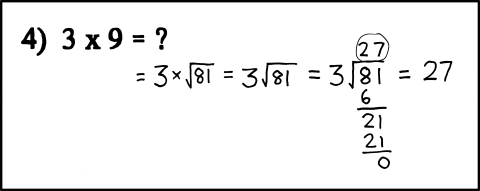
\includegraphics[width=0.5\textwidth]{3x9}\\
  \small{\textit{Image from \url{http://xkcd.com/759/}, CC BY-NC 2.5}}
\end{center}

\end{document}
